%%%%%%%%%%%%%%%%%%%%%%%%%%%%%%%%%%%%%%%%%%%%%%%%%%%%%%%%%%%%%
%% HEADER
%%%%%%%%%%%%%%%%%%%%%%%%%%%%%%%%%%%%%%%%%%%%%%%%%%%%%%%%%%%%%

\documentclass[a4paper, twocolumn, oneside, 11pt]{article}

\usepackage{fourier}
\usepackage[T1]{fontenc}

\usepackage{amssymb}
\usepackage{amsmath}
\usepackage{graphicx}
\usepackage{rotating}
\usepackage{pdflscape} 
\usepackage{abstract}
\usepackage[ table ]{ xcolor }
\usepackage[square, comma, sort&compress, longnamesfirst]{natbib} %
\usepackage{subfigure}
\usepackage{setspace}

\setlength{\marginparwidth}{3cm}
\usepackage{todonotes}
%\singlespacing %% 1-spacing (default)s
%\onehalfspacing
\newcommand{\degree}{$^{\circ}$\ }
%%% END Article customizations

%%% The "real" document content comes below...


\title{The saccadic flow baseline: Accounting for image-independent biases in fixation behaviour }

\author{Alasdair D. F. Clarke, Matthew J. Stainer, Benjamin W. Tatler \& Amelia R. Hunt}

\begin{document}

\twocolumn[
\maketitle
\begin{onecolabstract}
Much effort has been made to explain eye guidance during natural scene viewing. However, a substantial component of fixation placement appears to be a set of consistent biases in eye movement behaviour. We introduce the concept of \textit{saccadic flow}, a generalisation of the central bias that describes the image-independent conditional probability of making a saccade to $(x_{i+1},y_{i+1})$, given a fixation at $(x_i,y_i)$. We suggest that saccadic flow can be a useful prior when carrying out analyses of fixation locations, and can be used as a sub-module in models of eye movements during scene viewing. We demonstrate the utility of this idea by presenting bias-weighted gaze landscapes, and show that there is a link between the likelihood of a saccade under the flow model, and the salience of the following fixation. We also present a minor improvement to our central bias model (based on using a multivariate truncated Gaussian), and investigate the leftwards and coarse-to-fine biases in scene viewing. 
\end{onecolabstract}
]

%%%%%%%%%%%%%%%%%%%%%%%%%%%%%%%%%%%%%%%%%%%%%%%%%%%%%%%%%%
\section{Introduction}
%%%%%%%%%%%%%%%%%%%%%%%%%%%%%%%%%%%%%%%%%%%%%%%%%%%%%%%%%%

The human fovea provides a small window of high acuity vision to the world, and the locations that we select to view through this window can tell us how we seek the information necessary to complete the task we are currently undertaking. Fixation locations are selected based on a combination of low-level factors such as visual salience \citep{borji2013} and high-level factors \citep{yarbus1967, buswell1935, land2001}. However, there are also strong observable biases in eye movements that are independent of the content of the scene or the task being performed \citep{tatler-vincent2009, foulsham2010}, such as a strong tendency to fixate near to the centre of images \citep{tatler2007, canosa2003, stainer2013}. If we are to gain a complete understanding of the factors that govern how we sample information, we must build models of eye guidance on the framework of these underlying biases, using them as a baseline against which to compare effects of the scene, task, image properties and individual differences.

%%%%%%%%%%%%%%%%%%%%%%%%%%%%%%%%%%%%%%%%%%%%%%%%%%%%%%%%%%%%%
\subsection{Eye movement heuristics}
%%%%%%%%%%%%%%%%%%%%%%%%%%%%%%%%%%%%%%%%%%%%%%%%%%%%%%%%%%%%%

One influential model of eye movements of the last decade is the optimal search model \citep{najemnik-geisler2008}, which posits that human saccadic behaviour during visual search is consistent with predictions made by an ideal observer. The number of fixations human observers needed to make to find the target was closely matched by the ideal observer model, in which successive fixations were selected based on reducing uncertainty about the target's location, taking into account search history and target visibility across the visual field. The efficiency of human search (at least, in search for a Gabor patch hidden in $1/f$-noise) suggests this as a plausible mechanism for selecting fixations during search. Further evidence for this theory comes from \cite{ma2011} who found that human observers are near-optimal in a visual search task with line segments, and presented a neural network implementation of near-optimal search based on probabilistic population coding.  

While this modeling framework is attractive, there are several issues. The computations driving each fixation are complex, and depend on a fairly precise representation of one's own acuity over the visual field for a wide range of possible target/background combinations. One might therefore question the assumption that these computations are undertaken to determine the location of each of the 3-4 fixations made on average every second during visual search. More importantly,  \cite{morvan-maloney2012} demonstrated that human observers are not able to use information about visual sensitivity in the periphery to rationally plan even a single saccade to the optimal location in a target discrimination task. In their experiment, the observer simply has to select a location from which to detect a target that can appear with equal probability in one of two possible locations. If the locations are relatively close together, a location in between will maximise the probability of detecting a target appearing in either location. When the targets are too far apart to reliably detect the target from a point equidistant between them, the rational strategy is to look directly at one of the two possible target locations. Inconsistent with optimal viewing strategies, however, the observers did not systematically modify their choice about where to fixate according to the distance between the possible target locations. This striking failure of optimality has recently been replicated in a larger sample and generalized to other decisions in addition to eye movements \citep{clarke-hunt2015}. Further work from \cite{nowakowska2017} used a simple visual search display (an array of line segments) in which the target was easy to find (pop-out) when present in one half of the display, and hard to find when in the other. The optimal search strategy in this scenario is to search the difficult half of the display: if the target was present in the easy half, the observer would be able to find it using peripheral vision. While a minority of observers followed this search strategy, the majority exhibited large deviations, searching both halves equally, or even fixating the easy half and neglecting the difficult half of the display. These results are consistent with Morvan and Maloney’s explanation for the contradiction between their results and the predictions of Najemnik and Geisler’s optimal model: they propose that heuristics guide saccade planning. Heuristics include basic oculomotor biases such as a tendency to make saccades of particular amplitudes, and/or to particular regions of a display, or in particular sequences, depending on the current task. 

This idea has recently been formalised in a model by \cite{clarke2016}, who demonstrate that a stochastic search model based on a memoryless random walk can find a target in noise in a similar number of fixations to human observers. The key component of this model was the use of the empirical distribution of saccades: for each saccade the model randomly samples a saccade from distributions estimating the likelihood a human observer made a saccade from $(x_{i+1},y_{i+1})$ to $(x_i,y_i)$. It is clear from Figure \ref{fig:empiricalSaccadicFlow} that the distribution of saccade end points varies considerably depending on where the saccade is launched from. Thus a model that accounts for these launch-site dependent differences in exploration biases has the potential to offer a better account of viewing behaviour. This stochastic model differs from the random baseline implemented by \cite{najemnik-geisler2008}, in which they randomly selected each fixation location from all possible points in the display, because it incorporates basic oculomotor heuristics that guide the eyes, without the need for complex computation of peripheral sensitivity or target location probability. 

This stochastic search model is related to the more general topic of saccadic biases. Recent work in this area by \cite{leMeur-coutrot2016} independently arrived at a very similar model to \cite{clarke2016} while investigating context-dependent and spatially-variant viewing biases. Both their model and the Stochastic Search model partitioned the data into $k\times k$ subsets (\cite{leMeur-coutrot2016} used $k=3$ while \cite{clarke2016} used $k=5$) and then used non-parametric methods to model the distributions. In this paper, we re-implement and generalise this idea with a parameter named \textit{Saccadic Flow}, and examine the extent to which it is useful as a prior for analysing eye movements made with more natural (photographic) stimuli over a range of different tasks. 


\begin{figure}[htb]
\centering
\subfigure{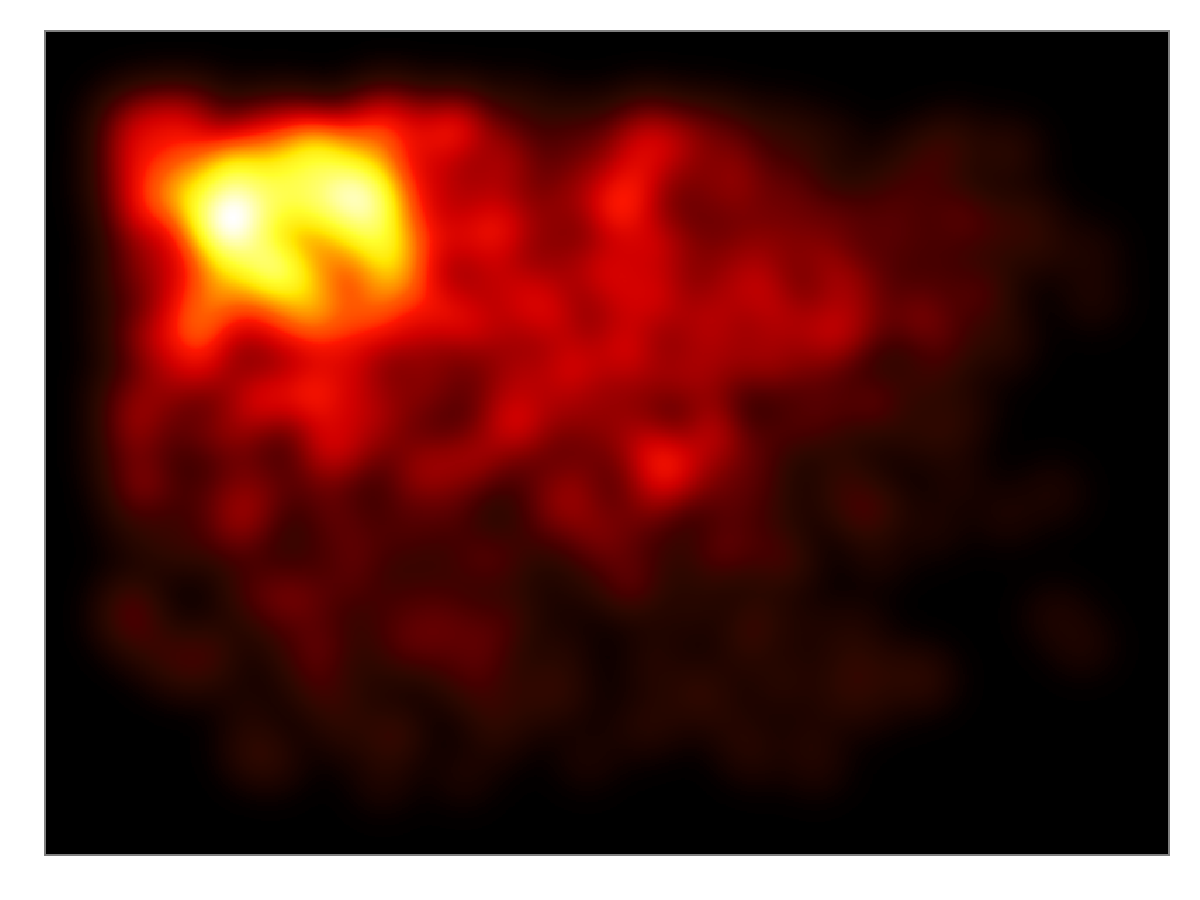
\includegraphics[width=2.5cm]{../scripts/heatmaps/SaccadicFlowMaps/Figures/BBias_11.pdf}}
\subfigure{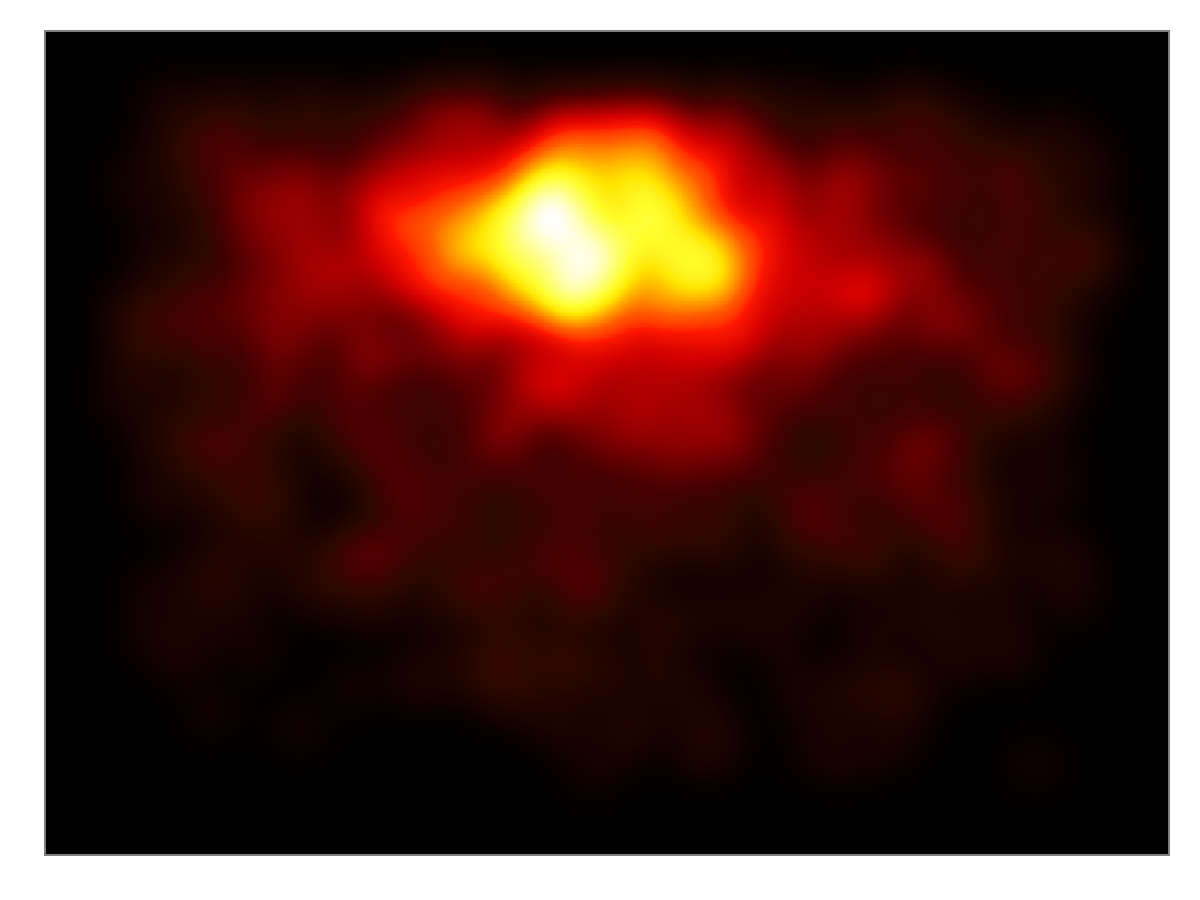
\includegraphics[width=2.5cm]{../scripts/heatmaps/SaccadicFlowMaps/Figures/BBias_12.pdf}}
\subfigure{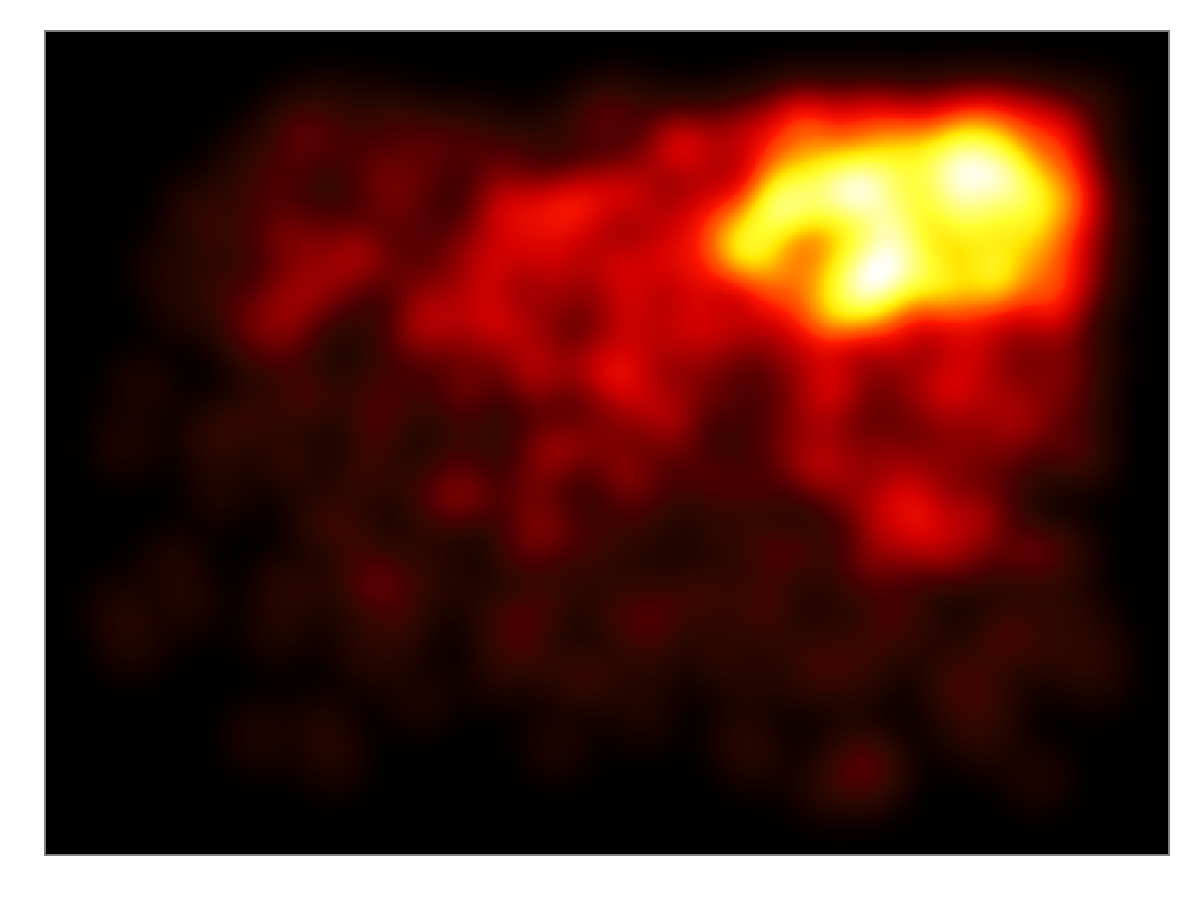
\includegraphics[width=2.5cm]{../scripts/heatmaps/SaccadicFlowMaps/Figures/BBias_13.pdf}}
\subfigure{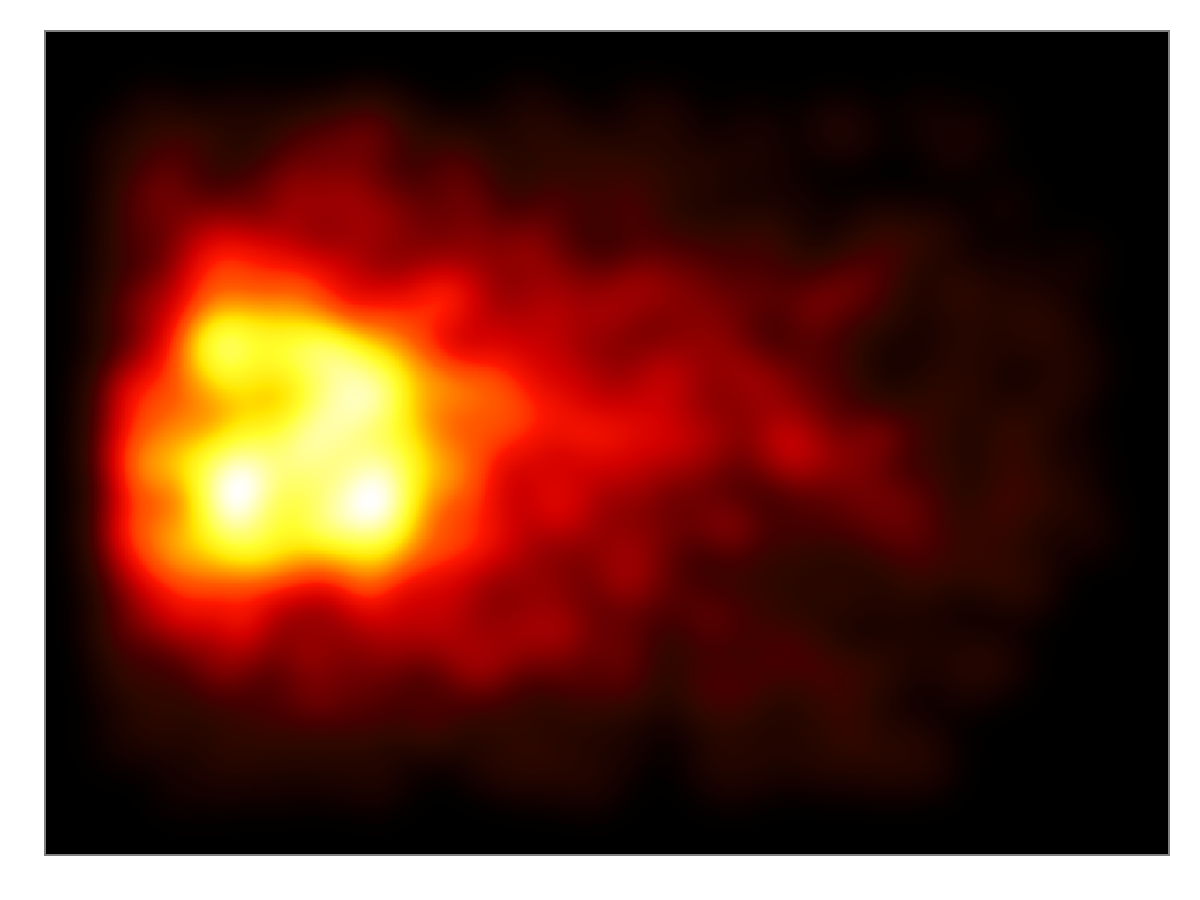
\includegraphics[width=2.5cm]{../scripts/heatmaps/SaccadicFlowMaps/Figures/BBias_21.pdf}}
\subfigure{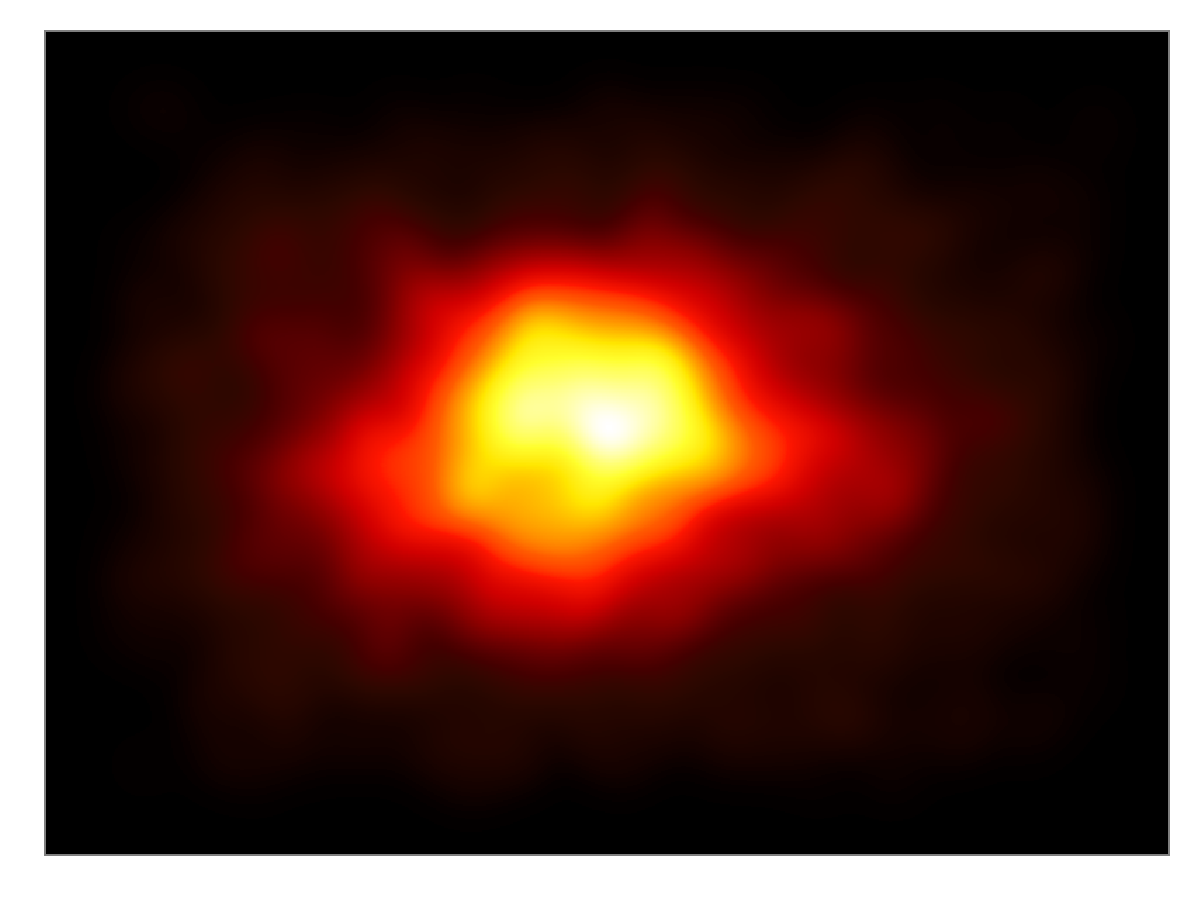
\includegraphics[width=2.5cm]{../scripts/heatmaps/SaccadicFlowMaps/Figures/BBias_22.pdf}}
\subfigure{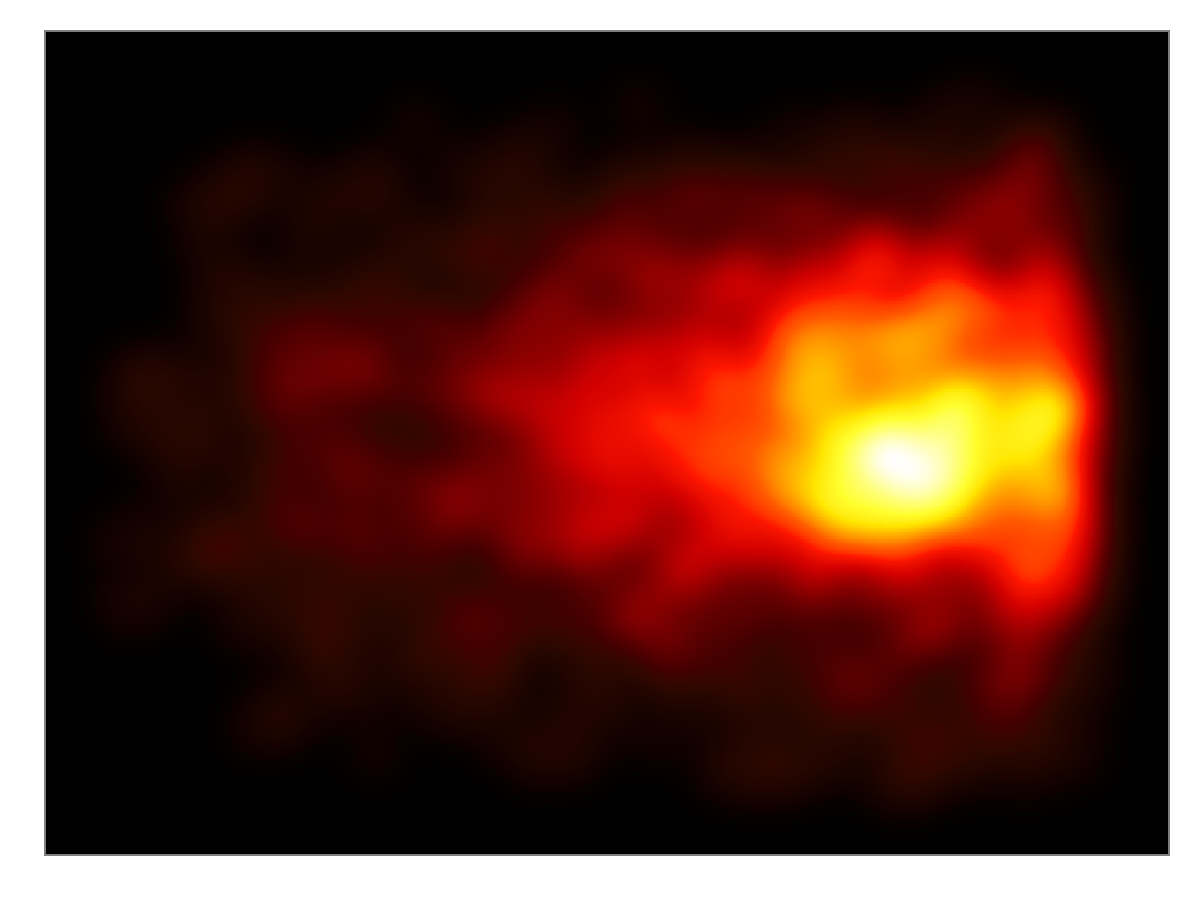
\includegraphics[width=2.5cm]{../scripts/heatmaps/SaccadicFlowMaps/Figures/BBias_23.pdf}}
\subfigure{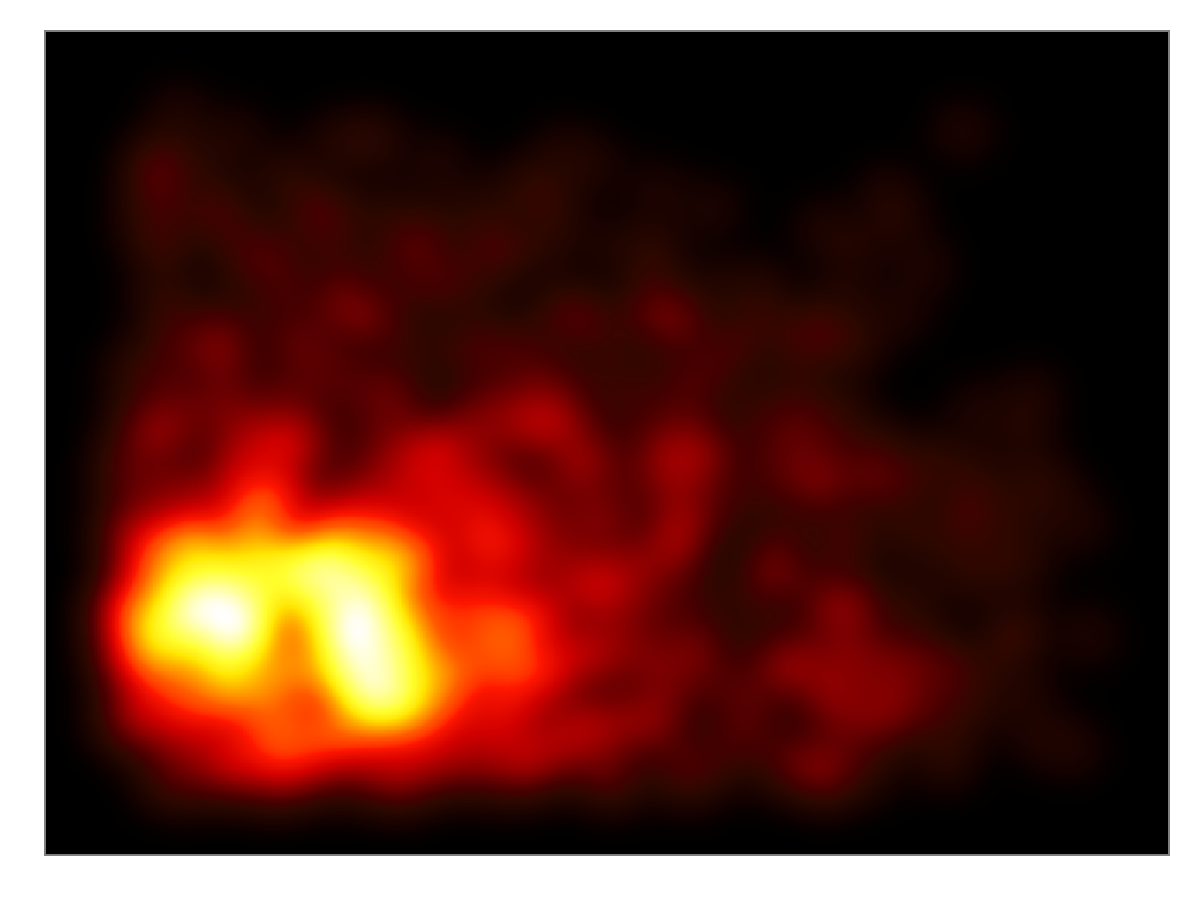
\includegraphics[width=2.5cm]{../scripts/heatmaps/SaccadicFlowMaps/Figures/BBias_31.pdf}}
\subfigure{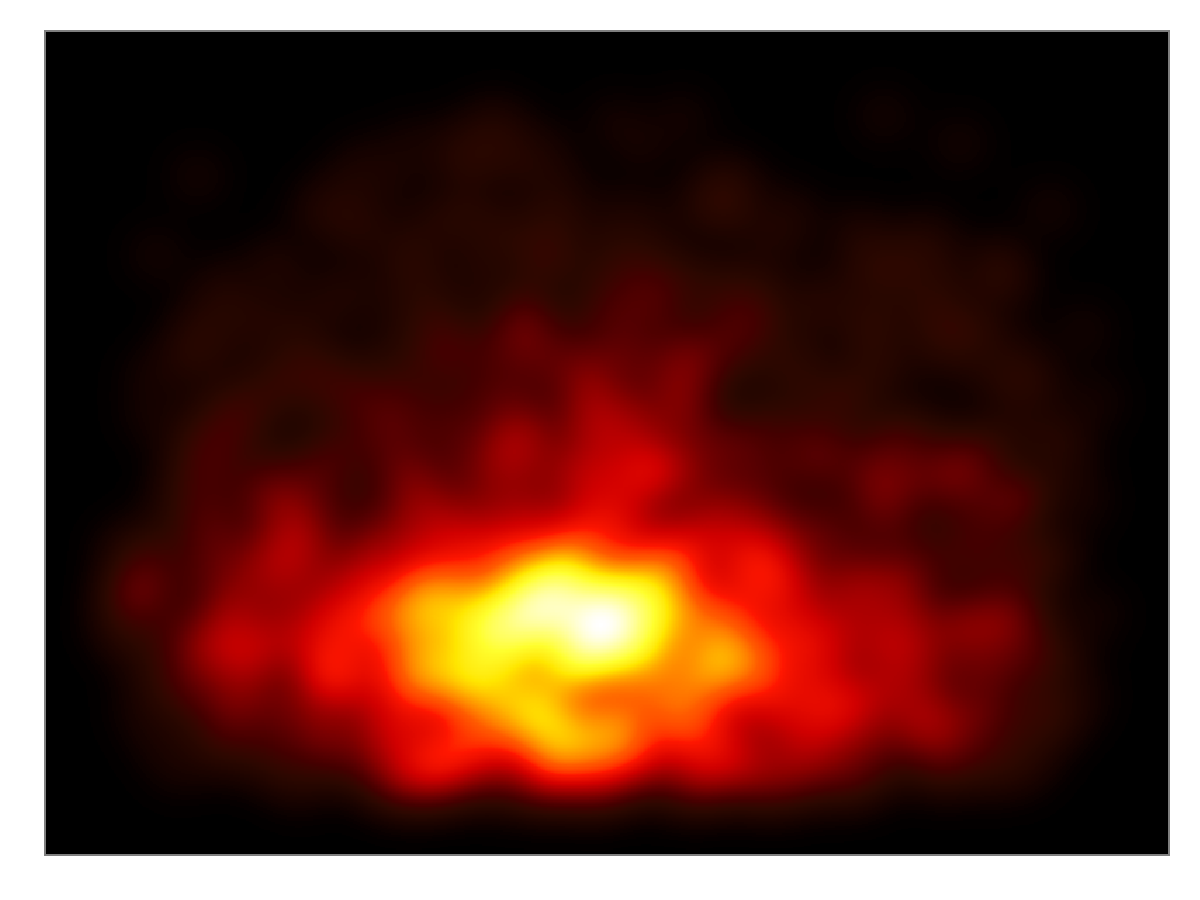
\includegraphics[width=2.5cm]{../scripts/heatmaps/SaccadicFlowMaps/Figures/BBias_32.pdf}}
\subfigure{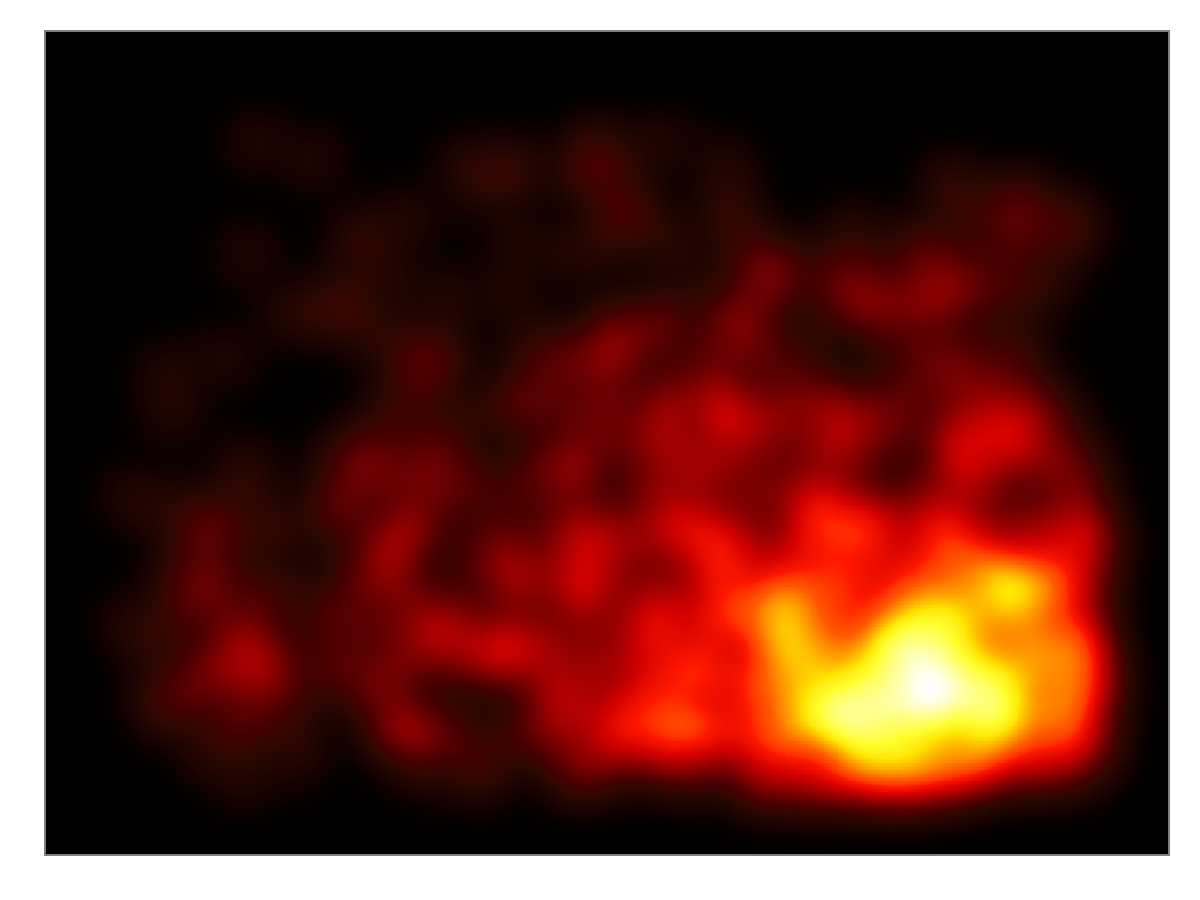
\includegraphics[width=2.5cm]{../scripts/heatmaps/SaccadicFlowMaps/Figures/BBias_33.pdf}}
\caption{Saccade landing positions from fixations that were in different sections of the screen. Data from each plot has been separated into fixations in 9 spatial bins, with the screen being divided into thirds in both horizontal and vertical aspects.}
\label{fig:empiricalSaccadicFlow}
\end{figure}

%%%%%%%%%%%%%%%%%%%%%%%%%%%%%%%%%%%%%%%%%%%%%%%%%%%%%%%%%%%%%
\subsection{The central bias}
%%%%%%%%%%%%%%%%%%%%%%%%%%%%%%%%%%%%%%%%%%%%%%%%%%%%%%%%%%%%%
 
There is a strong tendency for people to look close to the centre of pictures \citep{tatler2007, tatler2005, canosa2003, clarke-tatler2014} and videos \citep{tseng2009,loschky2015} presented on computer screens. There have been a number of suggestions for why this might be, the simplest being that the centre of the stimulus array is the best place to look to make use of parafoveal vision. Another possible explanation for this effect is that the muscles of the eye show a preference for the `straight ahead' position, re-centring in the orbit of the eye socket for most comfortable contraction of the ocular muscles (an \emph{orbital reserve} \citep{fuller1996}). As most scene viewing experimental set-ups stabilise the head to increase the accuracy of the eye tracking, and most scenes are presented in the centre of computer displays, such a re-centring mechanism would mean that the centre of images would indeed be preferentially selected. However, when scenes are scrambled into four quadrants, fixations are located near to the centre of each quadrant, rather than the display centre \citep{stainer2013}, suggesting that the central tendency is responsive to the scene itself rather than to the frame of the monitor upon which the scene is displayed. 

Another possible explanation for the central fixation bias is that it represents a response to \emph{photographer bias} in scenes, as photographers tend to frame their shots to include the most important content in the centre of the scene. However, when \cite{tatler2007} presented scenes where the image features were biased towards the edge of the scene, the central fixation bias persisted. The final possibility is that as a consequence of repeated exposure to photographer bias, the centre of scenes is simply where people are \emph{trained} to look at images \citep{parkhurst2002}. Such learning of spatial probabilities of targets can explain why, for example, people tend to look around the horizon when searching for people in natural scenes \citep{birmingham2009, torralba2006, ehinger2009}. Expecting to find interesting content in the centre of scenes might be a consequence of this hypothesis typically being correct. 

Irrespective of why it occurs, \cite{clarke-tatler2014} showed that the characteristics of the central bias are remarkably consistent across a series of eye movement databases over tasks such as free-viewing, visual search and object naming. They proposed a simple, standardised central baseline based on a multivariate Gaussian, and demonstrated that it outperforms similar measures previously used in the literature.

\subsection{Other behavioural biases in saccades}
While the central bias has attracted the most attention (at least in terms of models of visual attention), a number of other biases have been documented. These are discussed below. 

\textit{Horizontal Saccades}: Several researchers have noted that when viewing scenes there is a higher proportion of eye movements in horizontal directions than vertical or oblique movements \citep[e.g.][]{gilchrist2006,foulsham2008,tatler2008,lappe1998,lee2002}. There are a number of possibilities as to why this tendency exists. Firstly, there may be a muscular or neural dominance making oculomotor movements in the horizontal directions more likely. Secondly, the characteristics of photographic images may mean that content tends to be arranged horizontally by the photographer. In such situations, horizontal saccades may be the most efficient way to inspect scenes. Thirdly, using horizontal saccades in scene viewing might be a learned strategy. Observers may learn the natural characteristics of scenes based on previous experience, and therefore demonstrate an increased likelihood of moving in the horizontal direction. A final explanation is that this tendency is a consequence of the aspect ratio of visual displays, which normally allow for larger amplitude saccades in the horizontal than vertical directions \citep{wartburg2007}.

Results from Foulsham and colleagues suggest that the outline of the displayed scene has a marked effect on saccade directions during viewing. Indeed, \cite{foulsham2008} found that when the orientation of an image is rotated, the distribution of saccade directions follows the orientation of the scene. Furthermore, when a scene is presented in a circular aperture, the tendency to make horizontal saccades disappears, being replaced by a tendency to make vertical saccades relative to the image orientation \citep{foulsham-kingstone2010}. However, when using fractal images (where images do not have an obvious orientation), observers tend make horizontal saccades, regardless of the angle that the image is presented. These findings suggest that directional biases in saccades are not only influenced by the shape of the displayed scene but also its content.

\textit{Coarse-to-fine}: Another robust pattern in human saccadic behaviour is the tendency to make large eye movements after the initial scene onset, and smaller saccades as the trial unfolds \citep{over2007, pannasch2008,antes1974}. This is often accompanied by an increase in fixation durations,  and is framed as a move from ambient to focal processing \citep{follet2011,velichkovsky2002,unema2005}. \cite{godwin2014} successfully replicated these findings, but they offered an alternative explanation, namely that this behaviour is driven by stochastic factors that govern eye movements.

\textit{Leftwards bias}: Several studies have shown that observers exhibit a bias to fixate the left half of a stimulus over the right \citep{ossandon2014,nuthmann-matthias2014,learmonth2015,zelinsky1996, brandt1945}. This effect falls under the more general spatial attention bias of psuedoneglect \citep{bowers-heilman1980}, which also affects tasks such as line bisection. The leftwards bias is typically short-lived, affecting only the first couple of saccades after scene onset, and while it is robust, it is comparatively weak compared to other biases in scene viewing. For example,  \cite{dickinson-intraub2009} found $62\%$ of initial saccades were directed to the left half of the image during free viewing. There is some evidence that this bias is related to native reading direction \citep{friedrich2014}.

\textit{Saccadic Momentum and Inhibition of Return}: Several studies have described sequential dependencies during free viewing that bias saccades to repeat the same vector and amplitude (known as saccadic momentum) and to bias saccades away from returning to previously-visited targets (known as inhibition of return). Although both of these phenomena bias fixations away from previously-fixated locations, they differ in that inhibition of return is bound to a location in the search array, i.e. it is coded in object-based or spatiotopic coordinates (e.g. \cite{krueger-hunt2013}), while saccadic momentum has been characterised as a basic tendency to repeat the same motor program \citep{wang2011}. Inhibition of return, unlike saccadic momentum, is task-dependent \citep{dodd2009} and is disrupted by removing the scene or inhibited object  \citep{klein-macinnes1999, takeda-yagi2000}.  \cite{macinnes2014} observed both of these mechanisms operating during free visual search of a complex scene, but presumably only saccadic momentum would be consistently observed for all tasks and images. 

\subsection{The present study}

These biases, and in particular the central bias, are important to take into account when evaluating the performance of models of fixation location, and investigating relationships between eye movement data and other factors. The main contribution of this manuscript is to introduce the \textit{saccadic flow} model. This can be thought of as a generalisation of the central bias: instead of simply characterising the image-independent probability of fixating $(x_i, y_i)$ we model the conditional probabilities $p(x_i,y_i|x_{i-1}, y_{i-1})$. i.e. the probability of making a saccade from to $(x_i,y_i)$ given we are currently fixating $(x_{i-1}, y_{i-1})$.

In Section \ref{sec:biases} we describe the saccadic flow model and an improved version of the central bias model. The model's ability to account for eye movements during scene viewing is evaluated over 15 previously published datasets. These cover a range of types of images and viewing tasks. In Section \ref{sec:usingbiases} we demonstrate how the central bias and saccadic flow can be used to improve analysis and visualisation methods. In particular, we present bias-weighted gaze landscapes, and demonstrate an interaction between the likelihood of a saccade under different bias models and bottom-up visual salience. Finally, we investigate the short-comings of these generative models by comparing synthesised data to human eye movements. 




\section{Modelling Biases}
\label{sec:biases}

In this section, we (i) update the central bias model of \cite{clarke-tatler2014} to make use of a truncated Gaussian distribution that allows us to take the image boundaries into account; (ii) explore the strength of the leftwards bias in relation to the central bias; and (iii) describe the saccadic flow model. 


%%%%%%%%%%%%%%%%%%%%%%%%%%%%%%%%%%%%%%%%%%%%%%%%%%%%%%%%%%
\subsection{Modelling Methods}
\label{sec:modellingMethods}
%%%%%%%%%%%%%%%%%%%%%%%%%%%%%%%%%%%%%%%%%%%%%%%%%%%%%%%%%%

Here, we give an overview of the methods and data used for the saccadic flow modelling.

\subsubsection{Datasets}

We used a number of previously published datasets, covering a range of tasks, images, and experimental set-ups. This allow us to produce a model that will generalise well to other datasets. The models were trained on eight of the ten datasets used in \cite{clarke-tatler2014}. We chose to remove the data from \cite{asher2013} from our training set as the images have an aspect ratio of 5:4, whereas the rest of the data in our training set has an aspect ratio of 4:3. The pedestrian search dataset \citep{ehinger2009} was removed from the training set as previous analysis \citep{clarke-tatler2014} shows that it is biased compared to the other datasets analysed. Both of these datasets were used as test sets to evaluate how well our models generalise. 

We also added four new datasets to the ten used by \cite{clarke-tatler2014}. These were used to test the model. 

\begin{itemize}

\item \cite{jiang2014} collected data from 16 observers viewing 500 natural scenes containing crowds of people (aspect ratio 4:3).

\item \cite{clarke2009} investigated visual search for a target on a homogeneous textured background (i.e. target in noise). This dataset differs from the previous in that there is no semantic image content in the scene, and the stimuli had a 1:1 aspect ratio.

\item \cite{greene-wolfe2012} released a dataset of observers viewing square greyscale photographs.

\item \cite{borji2015} recently released a very large ($\approx 650,000$ fixations, 2000 images) dataset collected over twenty different stimulus types. Given the size of this dataset, and the wide-screen 16:9 aspect ratio, the evaluations on this dataset are presented separately, and split by stimulus class.
\end{itemize}
This gives us a relatively homogeneous training set, and a more heterogeneous test set. Hence, good performance on the test sets will likely be indicative of a generalisable result. An overview of the datasets used is given in Appendix Tables \ref{tab:datasets} and \ref{tab:setuptable}. 

\subsubsection{Pre-processing}

As with \cite{clarke-tatler2014}, we normalised all fixations to the image frame, keeping the aspect ratio constant. i.e., $(x,y)\in (-1.-1)\times(-a,a)$ with typically $a=0.75$. The initial saccades after image onset ($9.1\%$ of the data) were excluded, giving us a total of 159,226 saccades. Saccades with a start or end point falling outside of the image frame were also removed. 

When fitting saccadic flow models, we \textit{mirrored} the set of fixations, by adding in horizontally and vertically reflected copies of the data. This has two advantages. (i) It is an easy way to make the saccadic flow bias symmetric in the horizontal or vertical directions. This is similar to how the central bias was defined \cite{clarke-tatler2014}. (ii) It increases the amount of data available for fitting by a factor of four. This is important as (due to the central bias) there are relatively few saccades that originate from the corners of the images. By equating all corners, we can pool the data and obtain more stable estimates for the underlying distribution. The downside of mirroring saccades in this manner is that our model of saccadic flow will be insensitive to the \textit{leftwards bias} in natural scene viewing \citep{nuthmann-matthias2014}. However, as this accounts for a relatively small proportion of the overall variance in the data (Section \ref{sec:LeftRight}), we view this as an acceptable trade-off. Similarly, as we do not factor in the timecourse of the scanpath, we will not capture \textit{coarse-to-fine} dynamics (saccadic amplitude tends to decrease with time from stimulus onset).


\subsection{Truncated Central Bias}
\label{sec:truncatedCentral}

As the first step in modelling saccadic flow, we will update the central bias from \cite{clarke-tatler2014} and use a truncated normal distribution. This is straightforward. Re-fitting a multivariate Gaussian to the data reduces the deviance in the central bias model by $4.4\%$. Using a truncated Gaussian gives us an improvement of $12\%$. We can round the truncated Gaussian model to $\mu = (0,0)$, with a covariance matrix of $(0.32, 0; 0, 0.144)$ with no loss of precision. i.e. this is identical to \cite{clarke-tatler2014} except with $\sigma=0.32$ rather than $0.22$. We will use the abbreviations CT2014 and CT2017 to refer to these models.

\subsection{Left v Right}
\label{sec:LeftRight}

As mentioned above, the downside of mirroring the saccades in our dataset is that our bias model will be symmetric and will be unable to exhibit the leftward bias observed in human fixation data. Here, we investigate the size of the leftwards bias (in the unmirrored data) by plotting how the distribution of horizontal fixation location varies with fixation number (Figure \ref{fig:leftrightDist}). We can see that while we do have a leftwards bias in our data, it is a small effect that only last for the first five fixations after scene onset. Furthermore, there is no sign of an asymmetry in the vertical direction. Fitting an ANOVA to predict the $x$-coordinates of the fixations given the fixation number gives adjusted $R^2=0.004$. If we limit our analysis to the first five fixations in each scanpath, this only increases to adjusted $R^2=0.01$. The small size of the $R^2$ in both instances suggests that by ignoring the leftwards bias, we lose little explanatory power. This brings the advantage of then allowing us to treat everything as symmetrical, which simplifies the model and increases the amount of data available (by mirroring fixations). 

\begin{figure}
\centering
\subfigure{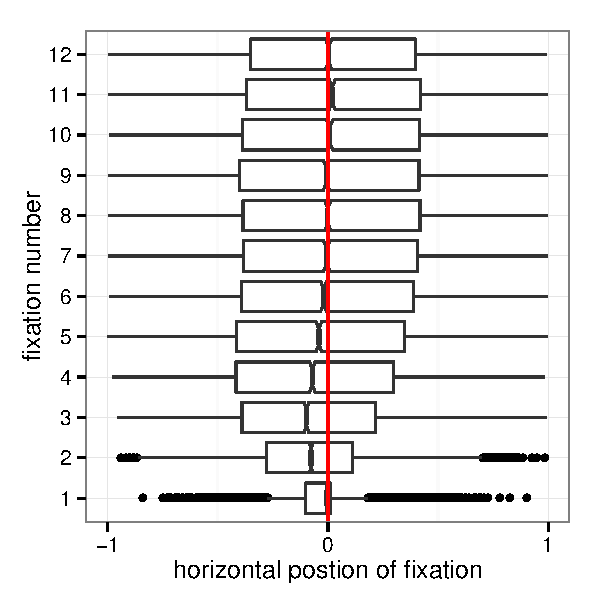
\includegraphics[width=3.8cm]{../scripts/leftVright/graphs/leftrightbias.pdf}}
\subfigure{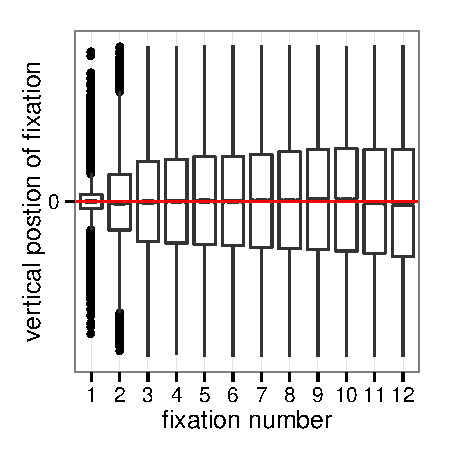
\includegraphics[width=3.8cm]{../scripts/leftVright/graphs/updownbias.pdf}}
\caption{Boxplots showing the distribution of horizontal and vertical fixations by fixation number in the merged training set}
\label{fig:leftrightDist}
\end{figure}


\subsection{Saccadic Flow}
\label{ModellingFlow}

Saccadic flow can be thought of as a generalisation of the central bias, and is illustrated in Figure \ref{fig:empiricalSaccadicFlow}. Instead of computing the distribution of all saccadic endpoints in a dataset, we look at the distribution of saccade endpoints given the start points, i.e., for a saccade from $(x_0, y_0)$ to $(x_1, y_1)$ we want to model $p(x_1,y_1|x_0, y_0)$.

\subsubsection{Modelling}

To characterise how the distribution of saccadic endpoints varies with the start point, we used a sliding window approach. All saccades that originated from a $n\times n$ window were taken and used to fit a truncated multivariate Gaussian distribution using the \texttt{tmvtnorm} library for \texttt{R}. This window was moved in steps of $s=0.01$ from $[-1,-0.75]$ to $[1-n, a-n]$. Windows containing less than 250 datapoints were discarded. We experimented with varying the window size ($n\in\{0.05,0.1, 0.2\}$). However, as this parameter was found to have a negligible result, we only report the results for $n=0.05$.

Multivariate polynomial regression was then used to fit 4-th order polynomials to each of the parameters. As polynomial regression performs poorly in the presence of outliers, we will also use robust estimation (\texttt{rlm} from the \texttt{MASS} library). This will stop the model fits being overly influenced by outlier points from the image boundary. Figure \ref{fig:nParamsOverSpace} shows how the parameters for the truncated multivariate Gaussian distributions vary over horizontal position for a selection of vertical positions. The regression coefficients (given in supplementary materials) allow us to estimate the conditional probability of a saccade to $(x_1, y_1)$ given the starting fixation $(x_0, y_0)$. As the robust estimation methods give a far better fit to the data, we will use this version of the model and discard the polynomial regression version.

\begin{figure*}[ht]
\centering
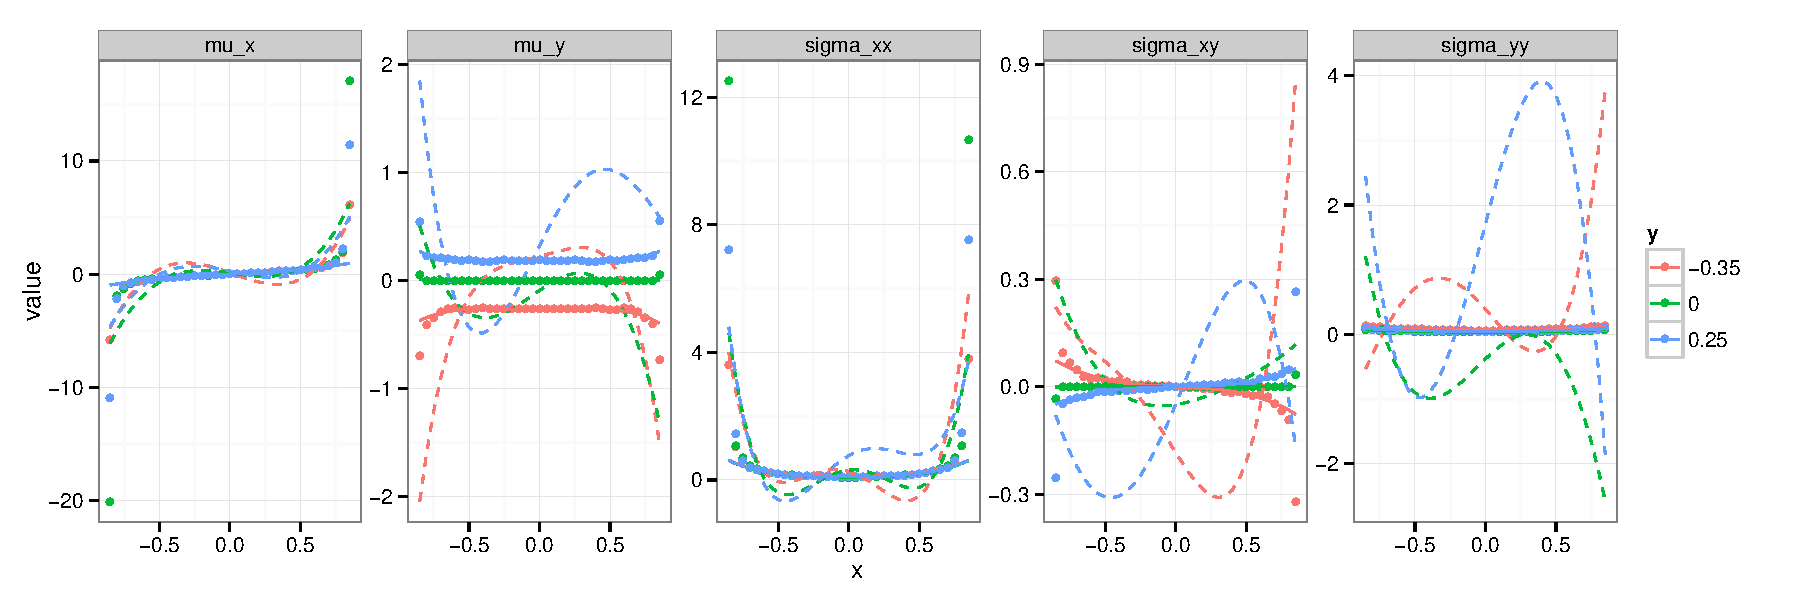
\includegraphics[width=13cm]{../scripts/flow/figs/NparamsChagingOverSpace_ALL_tN}
\caption{How the truncated Gaussian parameters vary with saccadic starting location. Dotted line show polynomial regression fits, solid line shows robust polynomial regression.}
\label{fig:nParamsOverSpace}
\end{figure*}

Evaluation will be done using bootstrapping (100 repetitions with $N=1000$). Not only does  this allow for confidence intervals to be estimated for our result, but it also allows us to sidestep the problems of using datasets of very different sizes: likelihood scores are heavily influenced by the number of points included in the analysis, so having this fixed at $N=1000$ means we can compare across datasets more meaningfully. We chose to evaluate how well the various models work by simply calculating the likelihood, $p(\text{data}|\text{model})$, for each dataset, and reporting the difference in log likelihood between a uniform distribution and our models. As the number of datapoints is much larger than the number of parameters, log likelihood approximates AIC. We also report a receiver operator curve (ROC) \citep{green-swets1966} analysis in which we look at how often saccades land within the most likely $x\%$ of the prediction maps from the different bias models. This analysis was done on the complete datasets without bootstrapping.

\subsubsection{Results}

How well does this model account for the fixations in our datasets? Figures \ref{fig:nFlowDevAll} and \ref{fig:nFlowDevBorji} compare how well the different models out-perform a uniform distribution in terms of log-likelihood. We can see that in all cases, the flow model offers a much larger improvement over a uniform distribution than either central bias model. The differences between the two central biases is much smaller, but in general, we can see that using a truncated distribution (to correctly take the image bounderies into account) offers a small improvement over the \cite{clarke-tatler2014} bias. 

It is interesting to note that the flow model still does a good job of accounting for the distribution of saccades in datasets (those involving visual search) in which the central bias is outperformed (in terms of log-likelihood) by the uniform distribution: chiefly the data from \cite{clarke2009,asher2013,tatler2007}. We can see a very similar pattern of results in the ROC analyis in Figure \ref{fig:nFlowROC}.

\begin{figure}
\centering
\subfigure[][Training datasets]{ \includegraphics[width=7cm]{../scripts/flow/figs/llh_training.pdf}}
\subfigure[][Test datasets]{ \includegraphics[width=7cm]{../scripts/flow/figs/llh_testing.pdf}}
\caption{Modeling results. We can see that the the flow model offers a much larger improvement in terms of log-likelihood than either of the central bias models. This holds even in datasets which do not show a strong central bias.}
\label{fig:nFlowDevAll}
\end{figure}

\begin{figure}
\centering
\subfigure[][Training datasets]{ \includegraphics[width=7cm]{../scripts/flow/figs/llh_training_ROC.pdf}}
\subfigure[][Test datasets]{ \includegraphics[width=7cm]{../scripts/flow/figs/llh_testing_ROC.pdf}}
\caption{ROC analysis comparing the flow model to the central bias.}
\label{fig:nFlowROC}
\end{figure}


\subsubsection{The Effect of Task}

We now examine how the ability of saccadic flow to explain different scanpaths depends on the observers' task. We will make use of datasets from \cite{mills2011} and \cite{koehler2014}. To look at this we computed the mean log likelihood over each scan-path in these datasets (see Figure \ref{fig:taskLLH}). We can see that while task has a slight influence over the mean log likelihood for a scan-path, there is a large degree of overlap in the distributions. Additionally, we can see that the relative likelihood of scan-paths made during visual search compared to other tasks varies between datasets. These results suggest that at least for the datasets considered here, the extent to which saccadic flow is able to explain the observed scan paths is not strongly influenced by the observer's task.


\begin{figure*}
\centering
 \subfigure[][]{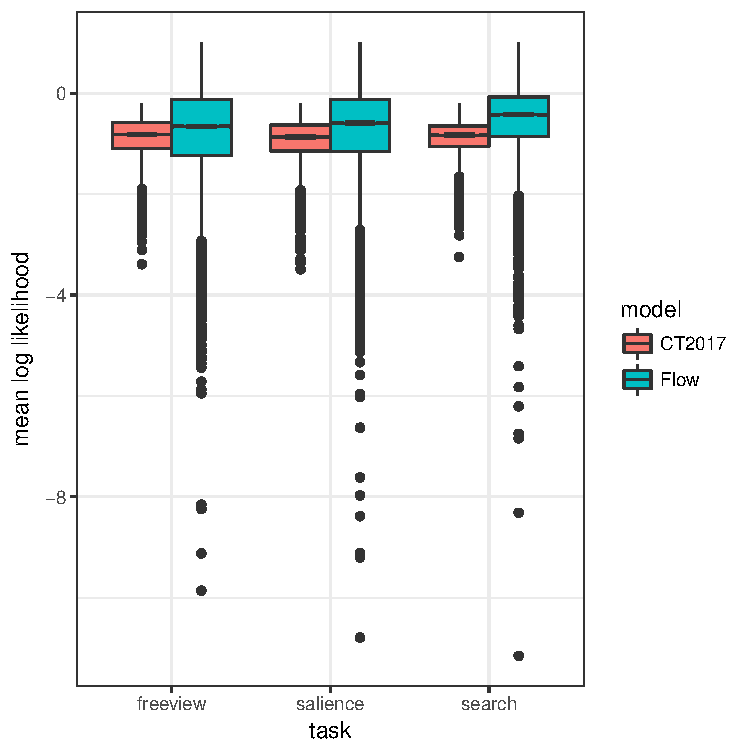
\includegraphics[width=5cm]{../scripts/inverseYarbus/kLLH.pdf}}
 \subfigure[][]{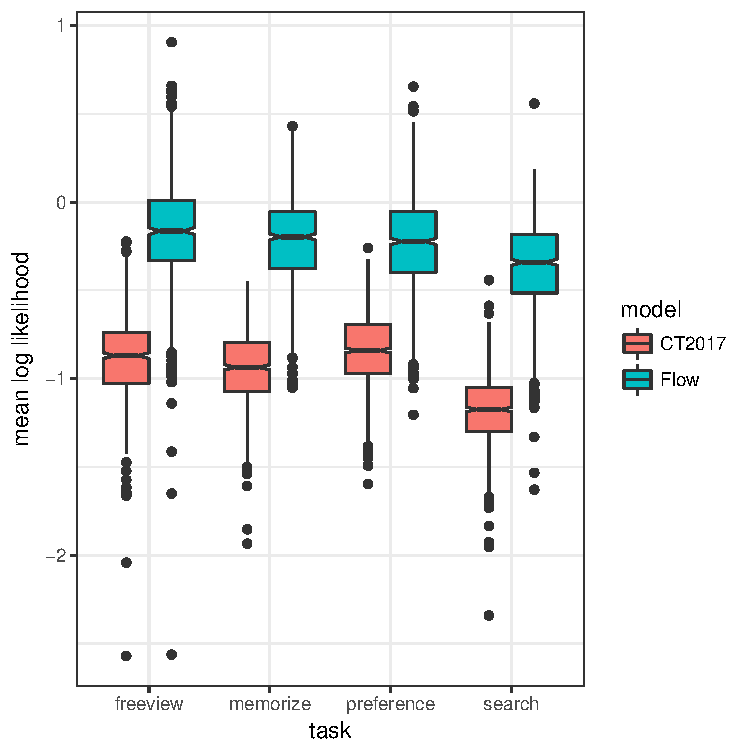
\includegraphics[width=5cm]{../scripts/inverseYarbus/millsLLH.pdf}}
\caption{The influence of task on the extent to which saccadic flow can explain scan-paths for the (a) \cite{koehler2014} and (b) \cite{mills2011} datasets.}
\label{fig:taskLLH}
\end{figure*}

\subsubsection{Saccadic flow and underlying physiology}
The saccadic flow model that we develop and evaluate here is a statistical model developed based on fitting empirical data. As such it does not make explicit any underlying physiological constraints or neurophysiological architecture. However, by constructing the model from observed data, these underlying constraints are necessarily present in the statistical model that we present here. The anisotropies in saccade directions that underlie the construction of the saccadic flow model are likely to reflect a combination of responses to the image and physiological constraints imposed by the arrangement and action of oculomotor muscles \cite{smit1987parametric,viviani1977curvature}. Similarly, the skew in saccade amplitudes toward favouring small amplitude saccades may reflect aspects of the drop-off in acuity limits with distance into the peripheral retina. Thus while these biomechanics and neurophysiological factors are not explicit in saccadic flow they necessarily inform the construction and thus any predictions arising from the model.


%%%%%%%%%%%%%%%%%%%%%%%%%%%%%%%%%%%%%%%%%%%%%%%%%%%%%%%%%%
\section{Using Biases}
\label{sec:usingbiases}
%%%%%%%%%%%%%%%%%%%%%%%%%%%%%%%%%%%%%%%%%%%%%%%%%%%%%%%%%%

This section makes use of an improved central bias model and the \textit{saccadic flow} model (described in Section \ref{ModellingFlow}). The new central bias model is similar to the model presented by \cite{clarke-tatler2014}, except for using a truncated Gaussian distribution to take the image boundaries into account. We present three examples of how these bias models can be used as priors in order to weight fixations, based on the fact that Flow produces likelihoods for any given fixation given the current fixation. First of all, we will demonstrate how we can weight fixations in gaze landscapes (also known as hotspot maps or heatmaps) to reduce noise and to give an improved visualisation of the image regions participants looked at more than expected. Secondly, we examine whether saccadic flow can be used to better understand the contribution of low-level features on fixation selection, and potentially lead to better evaluation of such computational saliency models. Finally, we demonstrate how flow can be used to generate a series of saccades, and compare these to observed human saccades. Being able to generate realistic synthetic datasets is useful to create an image-independent baseline with which to examine spatial maps of prediction using signal detection theory \citep[see][]{clarke-tatler2014}.

\subsection{Gaze landscapes}

One technique that is commonly used to visualise the spatial allocation of gaze is to create 'heatmap' plots where colour or luminance is used to indicate the density of fixation on those locations (Figure ~\ref{fig:adjustedHeatmaps}, column 2). A potential problem with visualising data in this way is that such maps represent all fixations as being of equal importance. For example, a location that is fixated for one second would be weighted equally with fixations that lasted half that time. If we want to make an assumption that fixation duration is intimately linked with the importance of that fixation (i.e. we will look longer at more informative information) then we can change our visualisation to weight fixations by their duration (Figure ~\ref{fig:adjustedHeatmaps}, column 3). \textbf{However, this weighted heatmap still fails to distinguish fixation behaviour likely to arise from image independent biases like the central fixation bias from fixation behaviour likely to reflect meaningful interrogation of, and response to, the viewed content.} 

\begin{figure*}
\centering
\includegraphics[width=13cm]{figs/heatmap_figure.pdf}
\caption{Examples of fixation heatmap plots from \cite{clarke2013}. The same fixations are presented where the Gaussian at each fixation is weighted by the duration of the fixation, the centre bias model from \cite{clarke-tatler2014} , and the saccadic flow model presented in this paper.}
\label{fig:adjustedHeatmaps}
\end{figure*}

An advantage of the \citet{clarke-tatler2014} model and the saccadic flow model presented here, is that we can represent fixations by the likelihood that they would occur based on the predictions of the models. Because the models reflect image-independent behavioural and oculomotor biases, fixations not predicted by these models might involve more high-level mechanisms. For example, given a tendency to fixate in the centre of the scene, we might consider saccades to non-central locations to be less predicted and therefore more likely to be image- or task-related.  In Figure ~\ref{fig:adjustedHeatmaps} (column 4 and 5) we present some overlaid heatmap data from the \citet{clarke2013} dataset, where fixations are weighted by the inverse probability of them occurring based on the models of central bias and saccadic flow. These figures reveal that representing data in this manner can allow us to visualise information that was important enough to disrupt these biases. In other words, these visualisations  remove some of the image-independent biases, and reveal the more important image \emph{dependent} information.


The top row of Figure ~\ref{fig:adjustedHeatmaps} demonstrates that weighting the fixations by the central bias and flow model both reduce the \emph{importance} of some fixations. The central bias model punishes fixations near the center of the image, while the flow model punishes fixations that were well predicted by the oculomotor biases of the saccadic flow model. Conversely, the models reward unlikely fixations. The second row reveals an instance of where the car to the left received less fixations than the pub sign, but that these fixations are boosted in the central bias and saccadic flow models where 'unlikely' saccades were made to this location. In the third and fourth rows, there are examples of images with important content near the centre of the photograph. This illustrates how the central bias model can sometimes over-compensate and reduce the influence of fixations in the centre of pictures that have important content located there. Given the tendency for photographers to centre their photographs around important content, reducing the weight of fixations to the castle in the painting (row 3) and the girl's face (row 4) would perhaps overly punish centrally biased photographic composition. With the flow model, however, these areas are still represented, as observers made saccades to theses regions that were unlikely to be driven by behavioural biases.

\subsection{Removing biases when examining image-dependent information}

By considering saccades in light of the probability that they were generated by image-independent biases, we can gain further insights into the image-dependent features that are important in attracting fixation. One feature that has been shown to correlate with fixation is visual salience \citep{parkhurst2002}. However, others have argued that this tendency is driven by the correlation between salient objects and their semantic interest \citep{henderson2007}, with interesting objects tending to be placed near to the centre of photographs \citep{tatler2007}. Oculomotor biases which favour a central tendency would predict the same fixation placement regardless of the distribution of salient objects in the image \citep{tatler-vincent2009}. Here, we can examine this question by looking at the relationship between saccade probability and the ability of different conspicuity maps to predict fixation. We can therefore examine how the effect of visual salience observed in eye movement analysis is related to the behavioural biases of eye movements.

We compared the proportion of fixations that fell in the brightest 20\% of pixels for salience maps to the likelihood of fixations from the flow and central bias models. Fixations were separated for each image into bins of 5\% from the least-likely to the most-likely to be generated based on salience. We then examined what proportion of each of these bins were in the brightest 20\% of salience maps using the Adaptive Whitening Saliency (AWS; \cite{garciadiaz2012}), RARE \citep{riche2013} and Graph-based visual saliency \citep[GBVS;][]{harel2006} algorithms. We selected AWS and RARE as they are the two best performing salience models according to the MIT Saliency Benchmark \citep{mit-saliency-benchmark,judd2012} with publicly available code, and GBVS as it contains a bias towards the centre cause by summing neighbouring pixel values across the spatial prediction map.

Figure ~\ref{fig:salmaps} reveals that the likelihood of making a saccade based on both the central bias and the flow model is highly related to salience in both AWS and RARE, with low-likelihood saccades being less likely to be to a salient region. Saccades that are very unlikely to be generated based on the oculomotor tendencies of eye movement (both flow and central bias) are therefore also less well explained by salience. Of the 5\% of fixations that were \textit{most} likely from saccadic flow, ~60\% of fixations fell in the 20\% thresholded region of the AWS map. However, of the 5\% of fixations that were \textit{least} likely from saccadic flow, only 40\% of fixations fell in this region. This means that it may be important to consider, and potentially remove, behavioural biases when attempting to predict fixation selection using feature-based models to ensure that any benefit in predictive power cannot be explained by behavioural biases correlating with salience. When examining a model that contains an inherent central bias (GBVS), we can see that weighting fixations by the \citet{clarke-tatler2014} central bias model is highly related to the performance of GBVS in predicting fixation selection.

%Examples of the maps can be seen in Figure \ref{fig:salmaps}. Salience maps were normalised to sum to 1, and data were analysed using linear mixed-effect models with the fixation weighting (duration, central bias or saccadic flow) as fixed effect factors, and image and participant as random effects. 

\begin{figure}
\centering
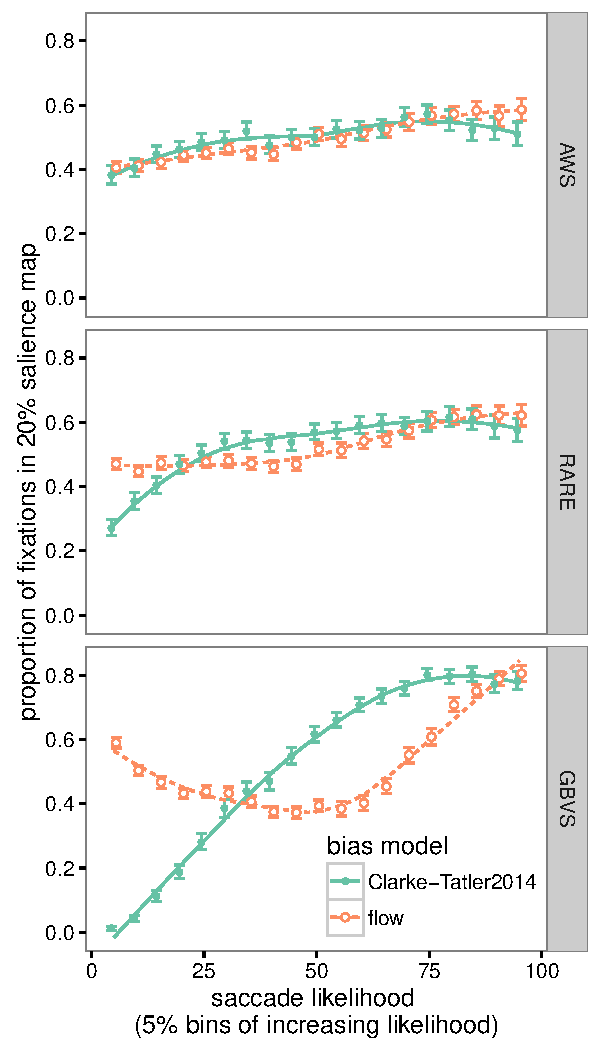
\includegraphics[width=\columnwidth]{figs/SaccadeSaliency.pdf}
\caption{Saccades binned by probability of them occurring in 5\% bins against the proportion of those fixations that fell in a 20\% thresholded region of AWS, RARE and GBVS salience maps.}
\label{fig:salmaps}
\end{figure}



\subsection{Saccadic Flow as a Generative Model}
\label{sec:humanComp}

Another use of the saccadic flow model is that it allows us to make spatial maps that relate to the probability of \emph{all saccades within a scene} based on the current position. For example, Figure~\ref{fig:flowPredict} shows that for three fixations in different locations within a scene, flow will make different spatial predictions of the next saccadic landing position. We can use this method to generate sequences of synthetic scan-paths. Here, we compare the distributions of these generated scan-paths with empirical scan-paths to determine which aspects of human saccadic behaviour are not captured by our model. To do this, we will create a merged dataset of fixations from the eight training datasets (175 000 fixations, including initial fixations, in total over 16 000 trials), and then generate a matched synthetic dataset such that the number of fixations in each trial is identical. 

\begin{figure*}[htb]
\centering
\subfigure[]{
\includegraphics[width=4.2cm]{figs/DownLeft.png}}
\subfigure[]{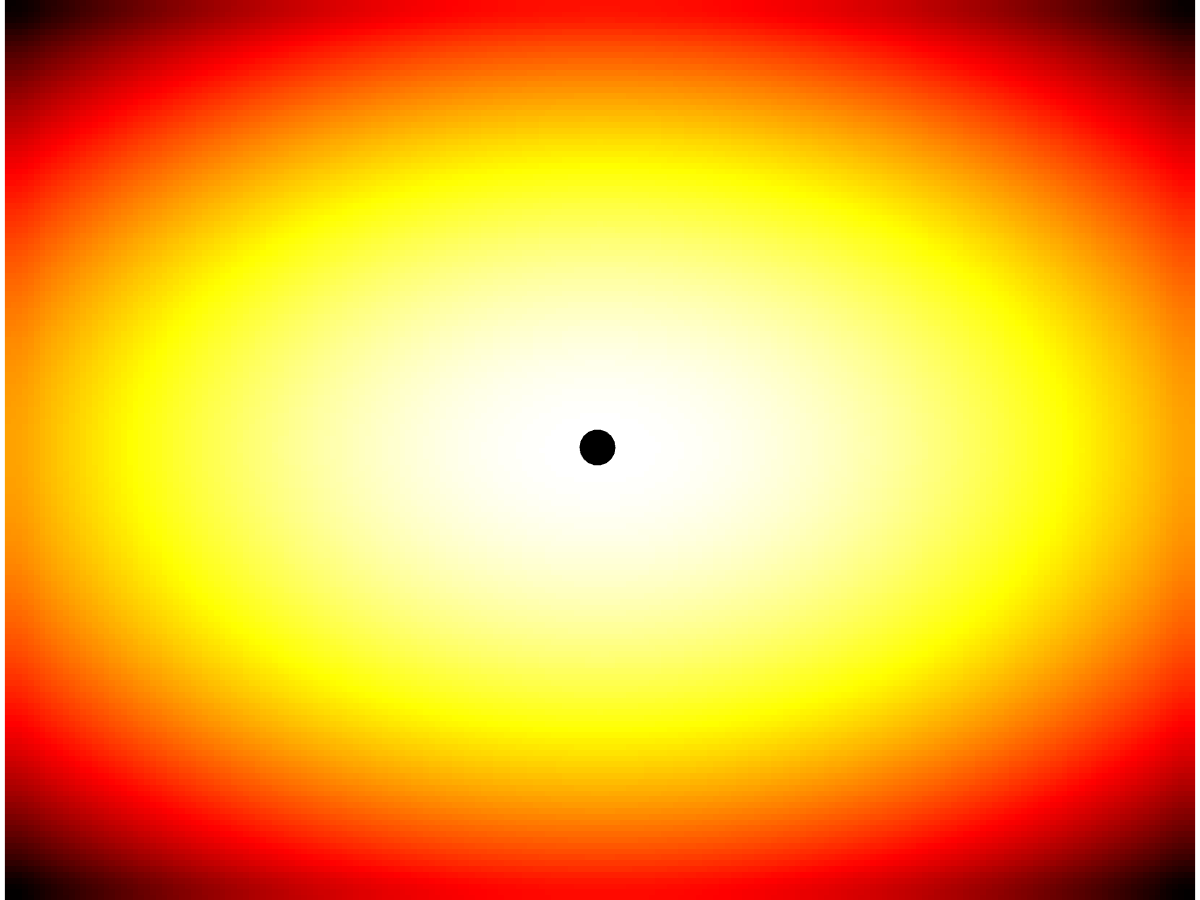
\includegraphics[width=4.2cm]{figs/Center.png}}
\subfigure[]{
\includegraphics[width=4.2cm]{figs/UpRight.png}}
\caption[]{Example spatial prediction maps for all potential saccade locations from 3 different fixation positions (black circles), to demonstrate how flow's predictions differ across the extent of a scene.}
\label{fig:flowPredict}
\end{figure*}

We can see from Figure \ref{fig:flowHumanComp}(a) and (b) that both the central bias and the saccadic flow model do a good job of capturing the distribution of fixation locations over the $x$ and $y$ axes. While it is not surprising that the central bias closely matches the empirical distributions (as this is exactly what it has been fitted to), it is interesting that saccadic flow does just as good a job. Hence, the central bias can be thought of as a property of saccadic flow, and does not need to be accounted for separately. 

When compared to the empirical distributions, both the central bias and saccadic flow appear to be slightly biased towards making fixations to the extreme edges of the image. This suggests that the truncated Gaussian distribution does not quite capture the effects of the image boundary on fixation selection and there is some additional aversion to fixating close to the screen edge. 

Another discrepancy between the synthetic and empirical distributions can be seen with saccadic amplitudes. While the flow model is a better fit to the human data than the central bias, it still underestimates the proportion of very short saccades (Figure \ref{fig:flowHumanComp}(c)). Interestingly, the flow model does manage to capture the initial increase in saccadic amplitudes after scene onset (Figure \ref{fig:flowHumanComp}(d)), but it does not explain the subsequent coarse-to-fine dynamics that are seen in the empirical scan-paths. 


\begin{figure}[htb]
\centering
\subfigure[]{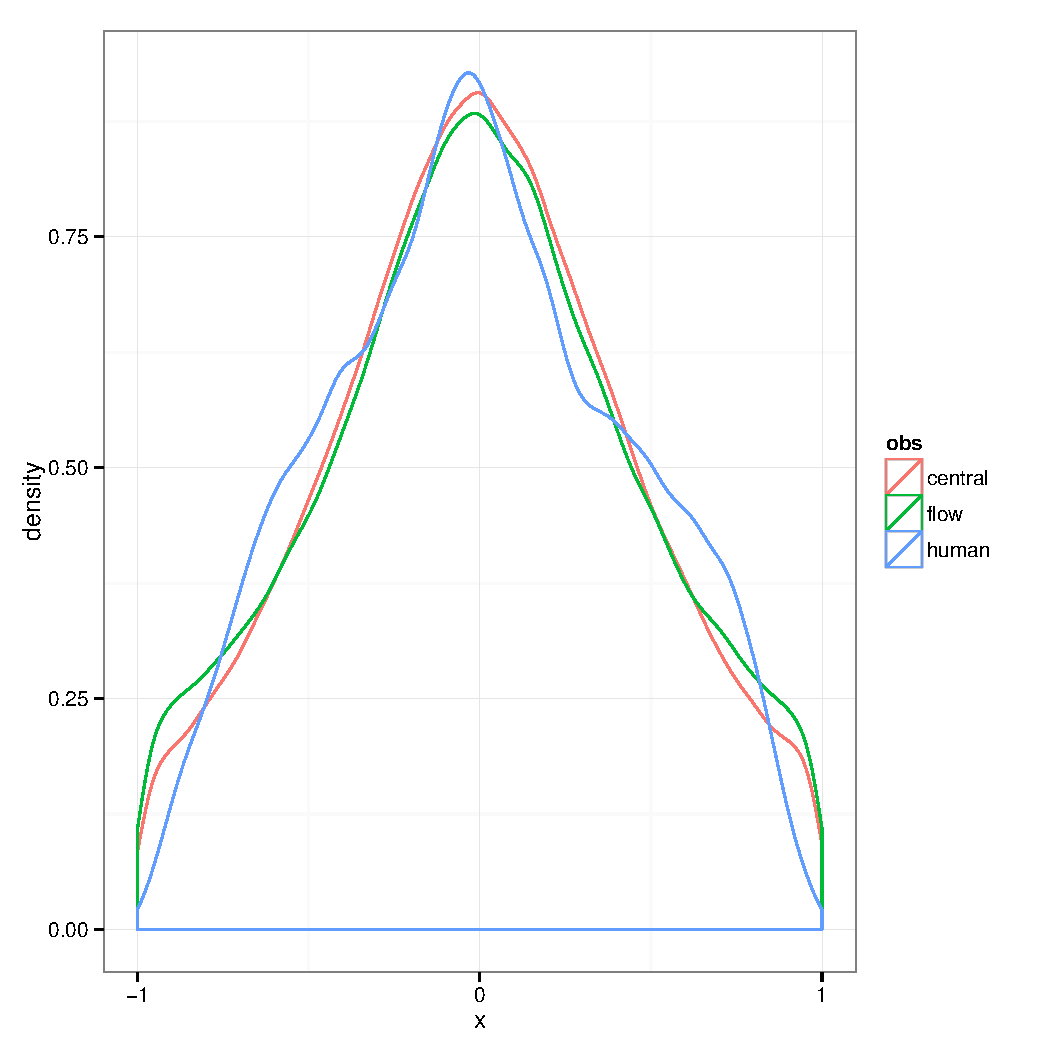
\includegraphics[width=3.8cm]{../scripts/coarse2fine/figs/xFixComparison}}
\subfigure[]{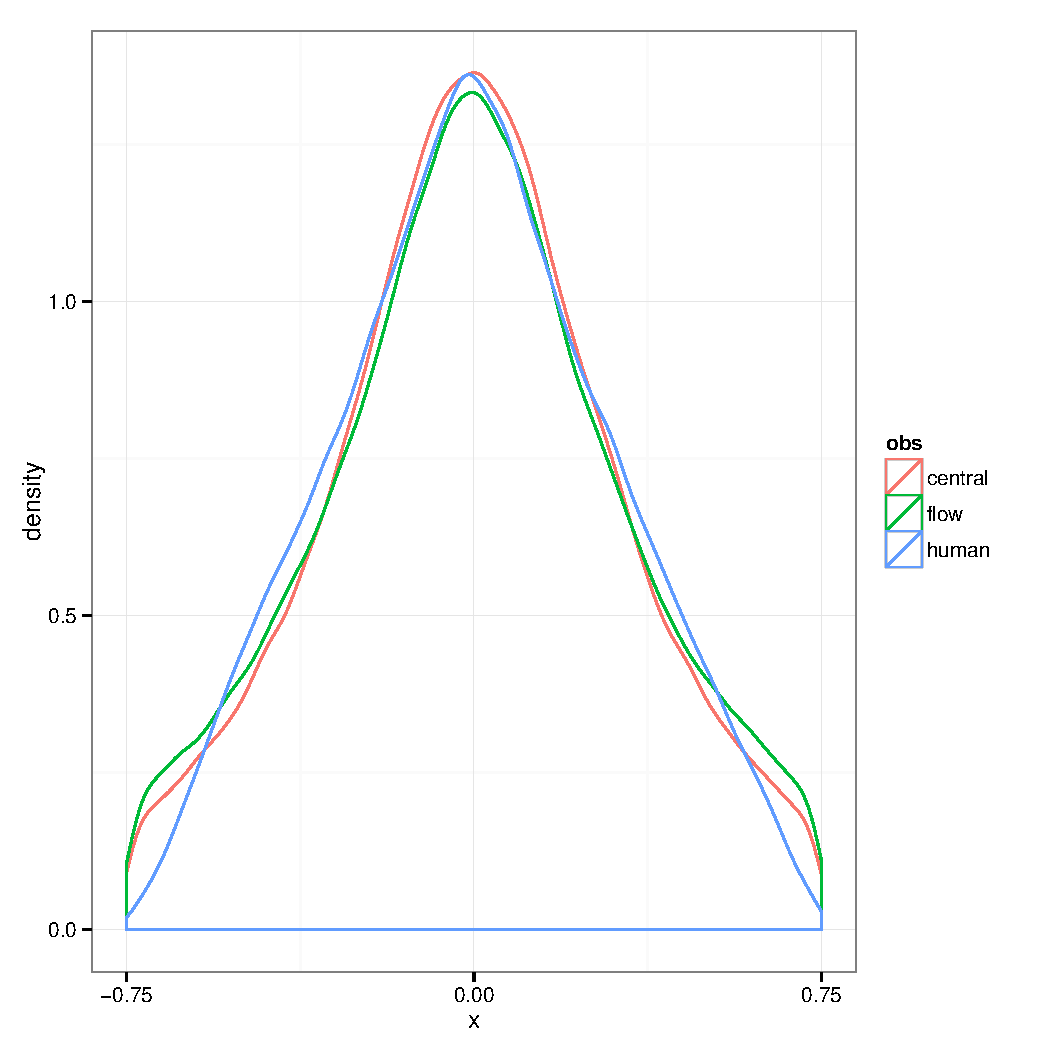
\includegraphics[width=3.8cm]{../scripts/coarse2fine/figs/yFixComparison}}
\subfigure[]{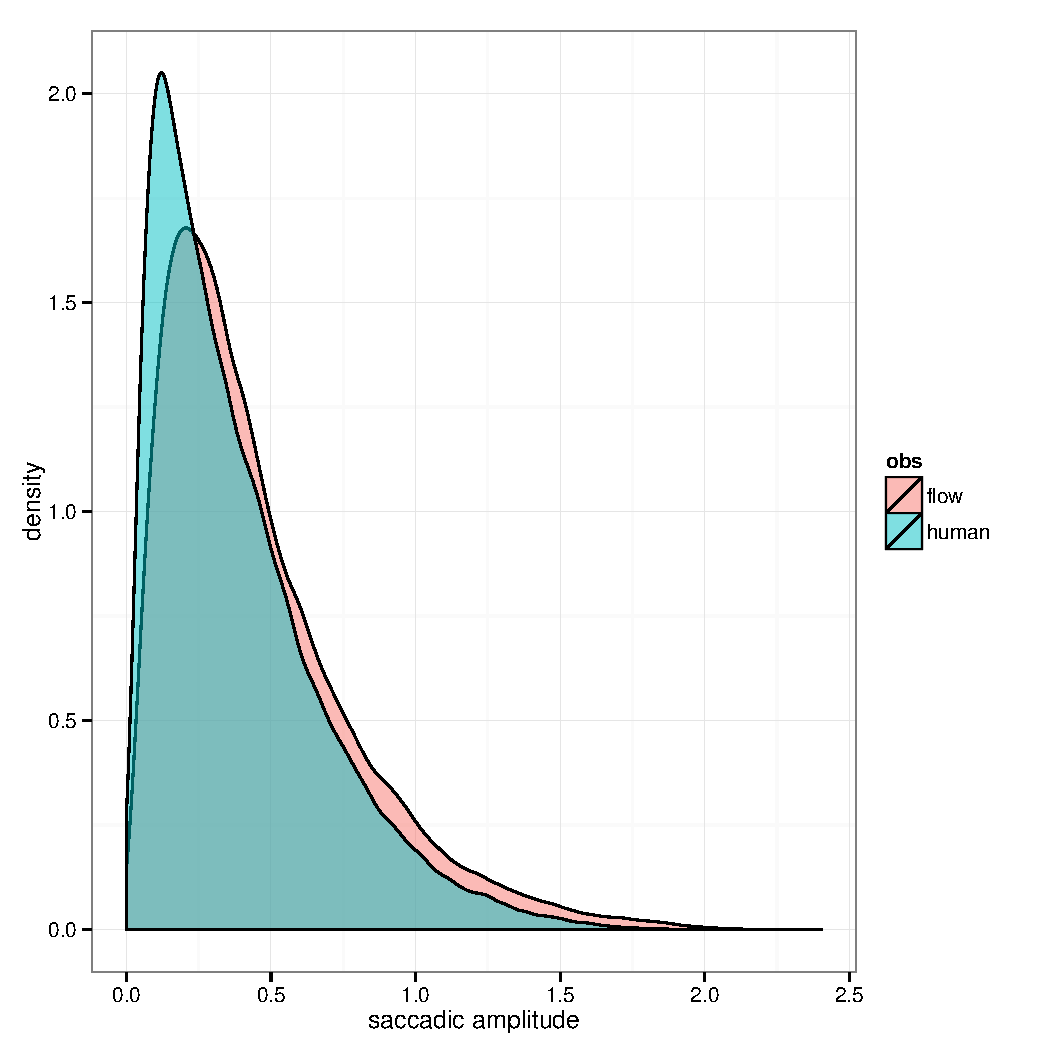
\includegraphics[width=3.8cm]{../scripts/coarse2fine/figs/ampSaccComparison}}
\subfigure[]{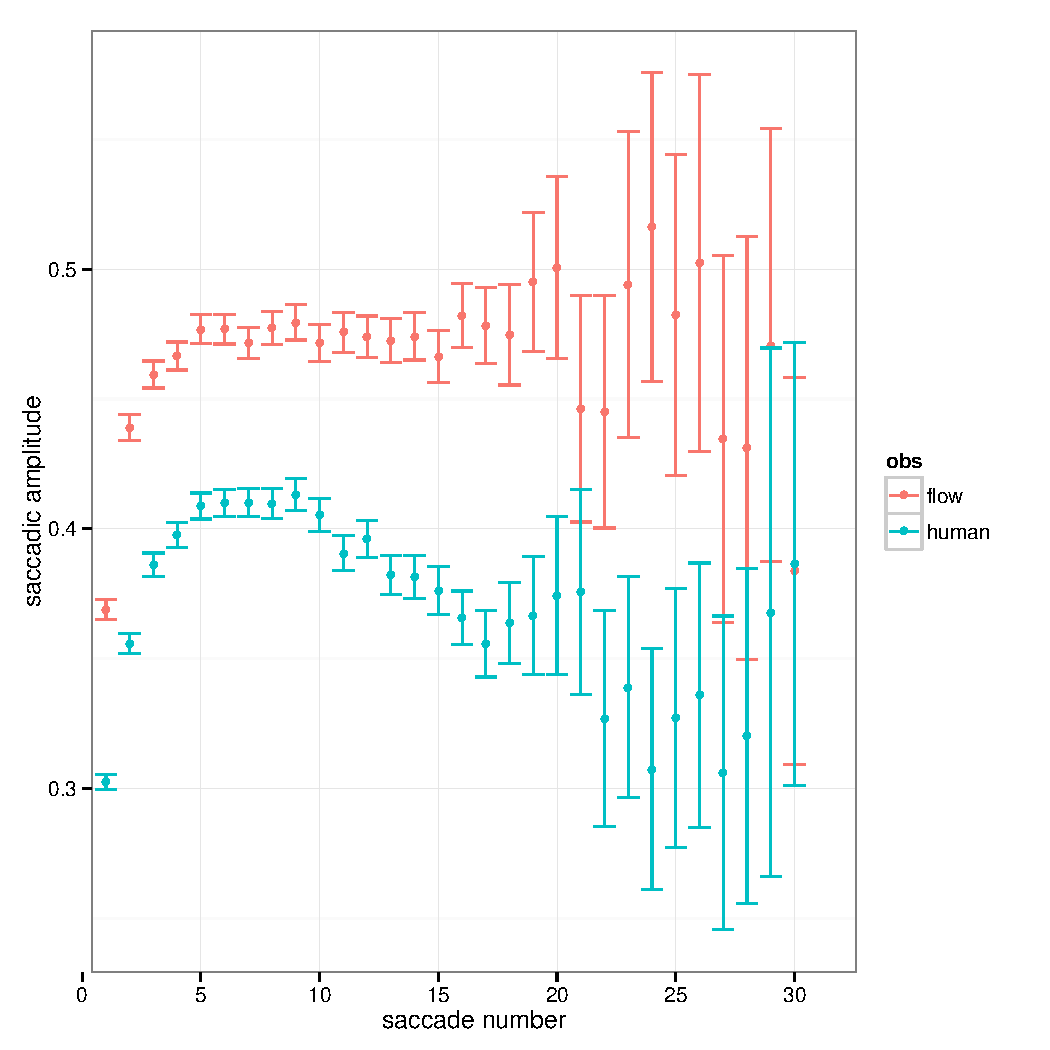
\includegraphics[width=3.8cm]{../scripts/coarse2fine/figs/saccAmpOverTimeFlow}}
\caption[]{\textit{blue}: human, \textit{red}: central bias, \textit{green}: saccadic flow. \textit{top row}: Comparison of $x$ and $y$ fixation positions between human fixations and synthetic points generated from the central bias and flow model. \textit{bottom row}: We can see that the flow model consistently makes saccades with a slightly larger amplitude than human observers. Distances are expressed relative to the width of the image. Best fit line in (d) fitted with loess regression. All distances are given in normalised units in which the width of an image is 2 (see Section \ref{sec:modellingMethods}).}
\label{fig:flowHumanComp}
\end{figure}


\subsection{Saccadic Flow across different tasks}


\subsection{Discussion}

We have demonstrated different ways biases such as saccadic flow and the central bias can be used in eye movement research. They can be used as a prior on the probability of making saccades to different regions of the image, allowing us to then more clearly visualise the image-dependant behaviour. We have also shown that the likelihoods of fixations under the bias models are related to features such as salience. The interpretation of visual salience as a predictive model of fixation selection can therefore be informed by considering how likely a saccade is to be generated by these models. Finally, we can also use the bias distributions to generate synthetic data that can be used as control points in ROC analysis, and to explore which aspects of human saccadic dynamics are not captured by the simple flow model. 
>>>>>>> Flow-2.0


\section{Discussion}

There has been much effort to generate a predictive model of human eye movements \citep{mit-saliency-benchmark,judd2009}. We propose the saccadic flow model as a robust prior for the image-independent saccadic behaviour that is evident when people look at pictures \citep{tatler-vincent2009}. Our Saccadic Flow model provides a better account of eye movement behaviour across 15 published datasets than the original Clarke and Tatler (2014) Central Bias model, and a new version of this model using truncated multivariate normal distributions. We find that Saccadic Flow accounts for eye movements across many different tasks and image types. As saccade probabilities across a scene can be predicted by Saccadic Flow, we therefore provide a method of modelling oculomotor biases that can be included in combined models of eye guidance, much as \cite{torralba2006} and \cite{ehinger2009} use context maps to predict where people will search for people.

\subsection{Using Saccadic Flow}
There are two ways in which models of eye movements may benefit from including such information. First, models may include saccadic flow in their calculation of spatial prediction. Understanding where someone is currently fixating in an image appears to dramatically influence where they will go next; as this saccadic flow can be parametrically estimated from any point on an image, it can be used to weight models of low-level (i.e. visual conspicuity) and high-level (i.e. semantic interest) features. Thus, whether someone fixates one of two equally conspicuous, equally interesting objects may be simply determined by the way that the eyes \textit{tend} to move. 

The second potential utility of saccadic flow is to generate realistic control fixations with which to evaluate observed fixation data. In this way, saccadic flow can be thought of as a partner to the \cite{clarke-tatler2014} central bias, and we expect that in some cases, the simpler central bias will be sufficient (for example, when examining the overall distribution of fixations rather than the sequence of saccades). However we have demonstrated that while the flow model requires more parameters (we use 16 coefficients to track how each of the five truncated Gaussian parameters vary as as a function of $(x,y)$ - although many of them are $\approx 0$), it generalises well from one dataset to another and is a far better baseline for modelling a scan-path than the central bias.

In the present paper, we have provided illustrative examples of how saccadic flow can be used to improve our understanding of eye guidance in scene viewing. Heatmaps that account for fixation likelihood under the behavioural biases captured in saccadic flow better reflect the image-dependent biases. Using these to base subsequent analysis of scene content at these locations or of differences in fixation behaviour under different tasks allows the researcher to focus analytical efforts on the viewing behaviour that is unlikely to arise from image-independent biases in how observers move their eyes. Given the prominence of image-independent biases in observed eye movement behaviour \cite{tatler-vincent2009}, removing these biases appropriately from analyses is important for effective evaluation of changes in behaviour arising from viewed content or behavioural task. Similarly, any attempt to model the involvement of factors such as image salience in eye guidance, should remove image-independent biases from modelling efforts in order to appropriately evaluate the role of any features under investigation. At present, the utility of removing the central bias from such modelling efforts is widely recognised \citep{borji2013,Tatler2011}, but we have shown in the present work that saccadic flow offers an even better explanation of underlying biases in fixation behaviour. Using saccadic flow to remove image-independent biases from datasets of eye movements will be an important improvement for testing existing models of fixation selection, and for better developing new models. Thus while the present work does not provide a direct answer to what factors govern scene inspection, it provides a vital tool for the field to allow this question to be addressed more effectively and appropriately than is currently possible.

\subsection{Comparisons to existing models}
\citep{tatler-vincent2009} have previously demonstrated that representing saccade probabilities based on the oculomotor biases in eye movements can account for human fixation behaviour during free-viewing reasonably well. Here we extend this concept to spatially adapt the prediction of saccade depending on where in a scene the preceding fixation lies. This is an important step, as it aligns the concept of behavioural biases in eye movement with the central bias \citep{tatler2007}, whereby saccades are likely to be directed towards the centre of the image. An advantage over the simpler central bias of Clarke and Tatler (2014) is that Saccadic Flow does not suppress fixations in the centre of the screen (where interesting content tends to lie), and sets of saccades generated from the Saccadic Flow model will produce the same centrally biased tendencies as observed fixations.

The work presented here improves on recent models by \cite{clarke2016,leMeur-coutrot2016} by offering a parametric model that avoids coarsely partitioning the data into large bins. We have demonstrated that the Saccadic Flow model generalises well to unseen test datasets, although this is likely to hold only for stimuli that are broadly similar to the images used to train the model (photographs of natural and manmade scenes). As we move away from photographic images to stimuli such as computer interfaces, we would expect the Flow model to offer a poor account of the data \citep{leMeur-coutrot2016}. While we have shown that the model performs well over a small range of tasks (free-viewing, scene description, object naming and visual search), we do observe differences in the log-likelihood when different tasks are carried out while viewing the same images. 

\subsection{Limitations of Saccadic Flow}

There are several limitations to our modelling work. Firstly, by using a truncated Gaussian we are unable to capture the skewed nature of the distribution of saccades originating from the corners (see Figure  \ref{fig:empiricalSaccadicFlow}). We experimented with fitting a skew-normal distribution using the \texttt{sn} package for \texttt{R}, but met with limited success due to having to deal with the image boundaries. We expect this is one of the reasons why our saccadic flow model generates saccades with an average greater amplitudes than those seen in empirical distributions.  The second simplification we make is to not take the leftwards biases in saccadic behaviour. However, our results suggest that this factor has a relatively small effect on saccades, and is important only for the first couple of saccades. Similarly, our model does not take into account coarse-to-fine biases. Across scene viewing, human fixations tend to increase in duration, and saccade amplitudes tend to decrease as the observer's understanding of the image changes \citep{antes1974}. Finally our model only considers the immediately preceding fixation as having an effect. This is likely to be an oversimplification of saccadic programming, given evidence in the literature that previous saccades and fixations influence saccade generation via processes such as saccadic momentum or inhibition of return \citep{macinnes2014}. With sufficient data, the modelling framework here could be extended to take the previous $n$ fixations into account. It should be noted, however, that the likely impact of these theoretical concepts upon the flow model is unclear: indeed failing to account for saccadic history may not be important for modelling some aspects of human search behaviour \citep{clarke2016}. The current implementation of saccadic flow also offers an opportunity to empirically assess the likely contribution of such factors as it offers a means to assess the likelihood of repeating a saccade (saccadic momentum) or returning to a previous location (inhibition of return).

\subsection{Conclusions}
Behavioural biases in eye movement are prevalent during scene viewing. Our saccadic flow model allows calculation of saccade likelihood across an image based on empirical data of how the eye tends to move in many different scene viewing conditions, with flow providing a strong fit to several datasets. There are a number of ways that flow can be developed, and we propose that gaining a better understanding of the saccadic biases underlying fixation behaviour can only be a positive for our search to understand why people look where they look. While the central bias model may be a better choice in some contexts, (i.e., when the analysis is in terms of unordered fixation coordinates), we recommend that using saccadic flow where possible. Flow consistently explains more variance than uniform and CT2014/17 models while also accounting for the central bias. This suggests that our model is robust, generalisable and should be of use to researchers interested in eye movements in a variety of scene-viewing paradigms. 


\section*{Acknowledgements}

This work was supported by the James S. McDonnell Foundation (Scholar Award to ARH).

\section*{Author Contribution}

All authors were involved in developing the ideas behind this work and co-wrote the paper. The saccadic flow model was developed by ADFC. The gaze landscapes and saliency analysis were done by MJS.

\appendix
\section{Dataset Details}

Here are all the details on the datasets used in this paper. (Table \ref{tab:datasets} and \ref{tab:setuptable}).


\begin{table*}
\centering
\small
\begin{tabular}{l|llll}
 						& Observers & Images &  Task & Display duration\\
\hline
\cite{clarke2013}     	& 24   	& 100   & object naming & 5000 ms\\
\cite{yun2013} - SUN    & 8     & 104   & image description & 5000 ms\\
\cite{tatler2005}     	& 14    & 48    & memory 			& variable\\
\cite{einhauser2008} 	& 8		& 93    & object naming 	& 3000 ms \\
\cite{tatler2007} - free & 22   & 120   & free viewing      & 5000 ms\\
\cite{judd2009}         & 15 	& 1003  & free viewing 		& 3000 ms\\
\cite{yun2013} - PASCAL & 3 	& 1000  & free viewing 		& 3000 ms\\
\cite{tatler2007} - search & 30 & 120	& visual search 	& 5000 ms\\
\hline
\cite{clarke2009} 		& 7		& 360	& visual search 	& variable\\
\cite{ehinger2009}     	& 14 	& 912 	& visual search 	& variable\\
\cite{asher2013}    	& 25    & 120   & visual search		& variable\\
\cite{jiang2014}  		& 16 	& 500 	& free viewing  	& 5000 ms \\
\cite{borji2015}  		& 120	& 4000  & free viewing		& 5000 ms\\
\end{tabular}

\caption{Summary of the 13 datasets used throughout this study. The top eight datasets were used to train the model, while the bottom five were only used for evaluation.}
\label{tab:datasets}
\end{table*}

\begin{table*}
\begin{center}
\small
\begin{tabular}{l|llllll}
 & Eye tracker & \vtop{\hbox{\strut Viewing}\hbox{\strut distance}}
 & \vtop{\hbox{\strut Screen}\hbox{\strut size}}
 & \vtop{\hbox{\strut Image}\hbox{\strut size}}
 & \vtop{\hbox{\strut Viewing}\hbox{\strut angle}}
 & \vtop{\hbox{\strut Chin /}\hbox{\strut head rest}}\\
\hline
\cite{tatler2005} 			& EyeLink I 	& 60 cm 	& 17" 	& $800 \times 600$ 	& $30 \times 22^{\circ}$ 	& no\\
\cite{tatler2007} - free 	& EyeLink II 	& 60 cm 	& 21" 	& $1600 \times 1200 $	& $40 \times 30^{\circ}$ 	& no \\
\cite{tatler2007} - search 	& EyeLink II 	& 60 cm 	& 21" 	& $1600 \times 1200$ 	& $40 \times 30^{\circ}$ 	& no\\
\cite{einhauser2008} 		& EyeLink 1000 	& 80 cm 	& 20" 	& $1024 \times 768$ 	& $29 \times 22^{\circ}$ 	& yes\\
\cite{judd2009} 			& ? 			& 2 feet 	& 19" 	& $1024 \times 768*$ 	& ? 				& yes\\
\cite{clarke2013} 			& EyeLink II 	& 50 cm 	& 21" 	& $800 \times 600$ 	& $31 \times 25^{\circ}$ 	& no\\
\cite{yun2013} - PASCAL 	& EyeLink 1000	& ? 		& ? 	& ? 			& ? 				& ?\\
\cite{yun2013} - SUN 		& EyeLink 1000 	& ? 		& ? 	& ? 			& ? 				& ?\\
\hline
\cite{clarke2009} 			& Tobii x50 	&87 cm			& 20"		& $1024\times 1024$	&	$16.7\times16.7^{\circ}$ & yes \\
\cite{ehinger2009} 			& ISCAN RK-464 	& 75 cm 	& 21" 	& $800 \times 600$ 	& $23.5 \times 17.7^{\circ}$& yes\\
\cite{asher2013} 			& EyeLink 1000 	& 55 cm 	& ? 	& $1024 \times 1280$& $37.6 \times 30.5^{\circ}$& yes\\
\cite{jiang2014}  			& Eyelink 1000 	& 57 cm		& 22"	& $1024 \times 768$ & $38.8 \times 29.1^{\circ}$& ?\\
\cite{borji2015} 			& Eyelink 1000	& 106 cm	& 42" 	& $1920\times1080 $	&$45.5\times31^{\circ}$& yes \\
\end{tabular}
\end{center}

\caption{Details of the experimental setups in each of the 10 datasets analysed in the present study. We provide only information reported in the original articles. Question marks indicate information not reported in the original article. *For the Judd et al dataset images varied in pixel dimensions but the majority were at 1024 x 768.}
\label{tab:setuptable}
\end{table*}


\section{Analysis of \cite{borji2015} dataset}

Here (Figure \ref{fig:nFlowDevBorji}) are the results for evaluating the flow model on the dataset from \cite{borji2015}.

\begin{figure*}
\centering
 \includegraphics[width=13cm]{../scripts/flow/figs/llh_trainingBorji.pdf}
\caption{Modeling results for the \cite{borji2015} data. We can see that the the flow model offers a much larger improvement in terms of log-likelihood than either of the central bias models.}
\label{fig:nFlowDevBorji}
\end{figure*}

\bibliographystyle{plainnat}
\small
\bibliography{literature.bib}
\end{document}
